\documentclass{ieeeaccess}
\usepackage{cite}
\usepackage{amsmath,amssymb,amsfonts}
\usepackage{algorithmic}
\usepackage{graphicx}
\usepackage{xcolor}
\usepackage{textcomp}
\usepackage{listings}
\usepackage{subfig}
\usepackage{braket}
\usepackage{hyperref}
\usepackage{cleveref}
\crefname{figure}{Figure}{Figures}
\crefname{section}{Section}{Sections}
\usepackage[htt]{hyphenat}



\def\BibTeX{{\rm B\kern-.05em{\sc i\kern-.025em b}\kern-.08em
    T\kern-.1667em\lower.7ex\hbox{E}\kern-.125emX}}
\begin{document}

\definecolor{codegreen}{rgb}{0,0.6,0}
\definecolor{codegray}{rgb}{0.5,0.5,0.5}
\definecolor{codepurple}{rgb}{0.58,0,0.82}
\definecolor{backcolour}{rgb}{0.95,0.95,0.92}

\lstdefinestyle{mystyle}{
  language=Python,
  basicstyle=\ttfamily\small,
  numbers=left,
  numberstyle=\tiny\color{codegray},
  stepnumber=1,
  numbersep=5pt,
  backgroundcolor=\color{white},
  showspaces=false,
  showstringspaces=false,
  showtabs=false,
  frame=single,
  rulecolor=\color{black},
  tabsize=2,
  captionpos=b,
  breaklines=true,
  breakatwhitespace=false,
  title=\lstname,
  keywordstyle=\color{blue},
  commentstyle=\color{codegreen},
  stringstyle=\color{red},
  escapeinside={\%*}{*)},
  morekeywords={*,...}
}

\lstset{style=mystyle}

\lstdefinelanguage{qoala}
{
    morekeywords=[1]{
        add, add, sub, addm, subm,
        jmp, bez, bnz, beq, bne, blt, bge,
        set, store, load
        meas,
        create_epr, recv_epr,
        init, meas, h, rot_x, rot_y, rot_z, cnot, cphase, cx_dir, cy_dir,
        APPID, NETQASM,
        run_request, run_routine, return_result, assign
    },
    morekeywords=[2]{
        META_START, META_END,
        SUBROUTINE,
        NETQASM_START, NETQASM_END,
        REQUEST
    },
    keywordstyle=[1]\color{blue},
    keywordstyle=[2]\color{purple},
    sensitive=true,
    morecomment=[l]{//},
    morecomment=[s]{/*}{*/},
    morecomment=[s][\color{blue}]{\#\ }{\ },
    morestring=[b]",
    escapeinside={(*@}{@*)},
}

\lstnewenvironment{qoalacode}{\lstset{style=mystyle,language=qoala}}{}

\newcommand{\revision}[1]{#1}
\newcommand{\todo}[1]{\textcolor{red}{TODO #1}}

\title{Qoala: an Application Execution Environment for Quantum Internet Nodes}

\author{
    Bart van der Vecht\authorrefmark{1,2,3},
    Atak Talay Yücel\authorrefmark{1},
    Hana Jirovská\authorrefmark{1,2,3},
    Stephanie Wehner\authorrefmark{1,2,3}
}
\address[1]{QuTech, Delft University of Technology}
\address[2]{Kavli Institute of Nanoscience, Delft University of Technology}
\address[3]{Quantum Computer Science, Electrical Engineering, Mathematics and Computer Science, Delft University of Technology}

\markboth
{Van der Vecht \headeretal: Qoala}
{Van der Vecht \headeretal: Qoala}

\corresp{Corresponding author: Bart van der Vecht (email: b.vandervecht@tudelft.nl).}

\begin{abstract}
Recently, a first-of-its-kind operating system for programmable quantum network nodes was developed, called QNodeOS.
Here, we present an extension of QNodeOS called Qoala, which introduces
(1) a unified program format for hybrid interactive classical-quantum programs, providing a well-defined target for compilers, and 
(2) a runtime representation of a program that allows joint scheduling of the hybrid classical-quantum program, multitasking, and asynchronous program execution.
Based on concrete design considerations, we put forward the architecture of Qoala, including the program structure and execution mechanism.
We implement Qoala in the form of a modular and extendible simulator that is validated against real-world quantum network hardware (available online).
However, Qoala is not meant to be purely a simulator, and implementation is planned on real hardware.
We evaluate Qoala's effectiveness and performance sensitivity to latencies and network schedules using an extensive simulation study.
Qoala provides a framework that opens the door for future computer science research into quantum network applications, including scheduling algorithms and compilation strategies that can now readily be explored using the framework and tools provided. 
\end{abstract}

\titlepgskip=-15pt

\maketitle

\section{Introduction}
\label{sec:introduction}
The business processes of organizations are experiencing ever-increasing complexity due to the large amount of data, high number of users, and high-tech devices involved \cite{martin2021pmopportunitieschallenges, beerepoot2023biggestbpmproblems}. This complexity may cause business processes to deviate from normal control flow due to unforeseen and disruptive anomalies \cite{adams2023proceddsriftdetection}. These control-flow anomalies manifest as unknown, skipped, and wrongly-ordered activities in the traces of event logs monitored from the execution of business processes \cite{ko2023adsystematicreview}. For the sake of clarity, let us consider an illustrative example of such anomalies. Figure \ref{FP_ANOMALIES} shows a so-called event log footprint, which captures the control flow relations of four activities of a hypothetical event log. In particular, this footprint captures the control-flow relations between activities \texttt{a}, \texttt{b}, \texttt{c} and \texttt{d}. These are the causal ($\rightarrow$) relation, concurrent ($\parallel$) relation, and other ($\#$) relations such as exclusivity or non-local dependency \cite{aalst2022pmhandbook}. In addition, on the right are six traces, of which five exhibit skipped, wrongly-ordered and unknown control-flow anomalies. For example, $\langle$\texttt{a b d}$\rangle$ has a skipped activity, which is \texttt{c}. Because of this skipped activity, the control-flow relation \texttt{b}$\,\#\,$\texttt{d} is violated, since \texttt{d} directly follows \texttt{b} in the anomalous trace.
\begin{figure}[!t]
\centering
\includegraphics[width=0.9\columnwidth]{images/FP_ANOMALIES.png}
\caption{An example event log footprint with six traces, of which five exhibit control-flow anomalies.}
\label{FP_ANOMALIES}
\end{figure}

\subsection{Control-flow anomaly detection}
Control-flow anomaly detection techniques aim to characterize the normal control flow from event logs and verify whether these deviations occur in new event logs \cite{ko2023adsystematicreview}. To develop control-flow anomaly detection techniques, \revision{process mining} has seen widespread adoption owing to process discovery and \revision{conformance checking}. On the one hand, process discovery is a set of algorithms that encode control-flow relations as a set of model elements and constraints according to a given modeling formalism \cite{aalst2022pmhandbook}; hereafter, we refer to the Petri net, a widespread modeling formalism. On the other hand, \revision{conformance checking} is an explainable set of algorithms that allows linking any deviations with the reference Petri net and providing the fitness measure, namely a measure of how much the Petri net fits the new event log \cite{aalst2022pmhandbook}. Many control-flow anomaly detection techniques based on \revision{conformance checking} (hereafter, \revision{conformance checking}-based techniques) use the fitness measure to determine whether an event log is anomalous \cite{bezerra2009pmad, bezerra2013adlogspais, myers2018icsadpm, pecchia2020applicationfailuresanalysispm}. 

The scientific literature also includes many \revision{conformance checking}-independent techniques for control-flow anomaly detection that combine specific types of trace encodings with machine/deep learning \cite{ko2023adsystematicreview, tavares2023pmtraceencoding}. Whereas these techniques are very effective, their explainability is challenging due to both the type of trace encoding employed and the machine/deep learning model used \cite{rawal2022trustworthyaiadvances,li2023explainablead}. Hence, in the following, we focus on the shortcomings of \revision{conformance checking}-based techniques to investigate whether it is possible to support the development of competitive control-flow anomaly detection techniques while maintaining the explainable nature of \revision{conformance checking}.
\begin{figure}[!t]
\centering
\includegraphics[width=\columnwidth]{images/HIGH_LEVEL_VIEW.png}
\caption{A high-level view of the proposed framework for combining \revision{process mining}-based feature extraction with dimensionality reduction for control-flow anomaly detection.}
\label{HIGH_LEVEL_VIEW}
\end{figure}

\subsection{Shortcomings of \revision{conformance checking}-based techniques}
Unfortunately, the detection effectiveness of \revision{conformance checking}-based techniques is affected by noisy data and low-quality Petri nets, which may be due to human errors in the modeling process or representational bias of process discovery algorithms \cite{bezerra2013adlogspais, pecchia2020applicationfailuresanalysispm, aalst2016pm}. Specifically, on the one hand, noisy data may introduce infrequent and deceptive control-flow relations that may result in inconsistent fitness measures, whereas, on the other hand, checking event logs against a low-quality Petri net could lead to an unreliable distribution of fitness measures. Nonetheless, such Petri nets can still be used as references to obtain insightful information for \revision{process mining}-based feature extraction, supporting the development of competitive and explainable \revision{conformance checking}-based techniques for control-flow anomaly detection despite the problems above. For example, a few works outline that token-based \revision{conformance checking} can be used for \revision{process mining}-based feature extraction to build tabular data and develop effective \revision{conformance checking}-based techniques for control-flow anomaly detection \cite{singh2022lapmsh, debenedictis2023dtadiiot}. However, to the best of our knowledge, the scientific literature lacks a structured proposal for \revision{process mining}-based feature extraction using the state-of-the-art \revision{conformance checking} variant, namely alignment-based \revision{conformance checking}.

\subsection{Contributions}
We propose a novel \revision{process mining}-based feature extraction approach with alignment-based \revision{conformance checking}. This variant aligns the deviating control flow with a reference Petri net; the resulting alignment can be inspected to extract additional statistics such as the number of times a given activity caused mismatches \cite{aalst2022pmhandbook}. We integrate this approach into a flexible and explainable framework for developing techniques for control-flow anomaly detection. The framework combines \revision{process mining}-based feature extraction and dimensionality reduction to handle high-dimensional feature sets, achieve detection effectiveness, and support explainability. Notably, in addition to our proposed \revision{process mining}-based feature extraction approach, the framework allows employing other approaches, enabling a fair comparison of multiple \revision{conformance checking}-based and \revision{conformance checking}-independent techniques for control-flow anomaly detection. Figure \ref{HIGH_LEVEL_VIEW} shows a high-level view of the framework. Business processes are monitored, and event logs obtained from the database of information systems. Subsequently, \revision{process mining}-based feature extraction is applied to these event logs and tabular data input to dimensionality reduction to identify control-flow anomalies. We apply several \revision{conformance checking}-based and \revision{conformance checking}-independent framework techniques to publicly available datasets, simulated data of a case study from railways, and real-world data of a case study from healthcare. We show that the framework techniques implementing our approach outperform the baseline \revision{conformance checking}-based techniques while maintaining the explainable nature of \revision{conformance checking}.

In summary, the contributions of this paper are as follows.
\begin{itemize}
    \item{
        A novel \revision{process mining}-based feature extraction approach to support the development of competitive and explainable \revision{conformance checking}-based techniques for control-flow anomaly detection.
    }
    \item{
        A flexible and explainable framework for developing techniques for control-flow anomaly detection using \revision{process mining}-based feature extraction and dimensionality reduction.
    }
    \item{
        Application to synthetic and real-world datasets of several \revision{conformance checking}-based and \revision{conformance checking}-independent framework techniques, evaluating their detection effectiveness and explainability.
    }
\end{itemize}

The rest of the paper is organized as follows.
\begin{itemize}
    \item Section \ref{sec:related_work} reviews the existing techniques for control-flow anomaly detection, categorizing them into \revision{conformance checking}-based and \revision{conformance checking}-independent techniques.
    \item Section \ref{sec:abccfe} provides the preliminaries of \revision{process mining} to establish the notation used throughout the paper, and delves into the details of the proposed \revision{process mining}-based feature extraction approach with alignment-based \revision{conformance checking}.
    \item Section \ref{sec:framework} describes the framework for developing \revision{conformance checking}-based and \revision{conformance checking}-independent techniques for control-flow anomaly detection that combine \revision{process mining}-based feature extraction and dimensionality reduction.
    \item Section \ref{sec:evaluation} presents the experiments conducted with multiple framework and baseline techniques using data from publicly available datasets and case studies.
    \item Section \ref{sec:conclusions} draws the conclusions and presents future work.
\end{itemize}
\section{RELATED WORK}
\label{sec:relatedwork}
In this section, we describe the previous works related to our proposal, which are divided into two parts. In Section~\ref{sec:relatedwork_exoplanet}, we present a review of approaches based on machine learning techniques for the detection of planetary transit signals. Section~\ref{sec:relatedwork_attention} provides an account of the approaches based on attention mechanisms applied in Astronomy.\par

\subsection{Exoplanet detection}
\label{sec:relatedwork_exoplanet}
Machine learning methods have achieved great performance for the automatic selection of exoplanet transit signals. One of the earliest applications of machine learning is a model named Autovetter \citep{MCcauliff}, which is a random forest (RF) model based on characteristics derived from Kepler pipeline statistics to classify exoplanet and false positive signals. Then, other studies emerged that also used supervised learning. \cite{mislis2016sidra} also used a RF, but unlike the work by \citet{MCcauliff}, they used simulated light curves and a box least square \citep[BLS;][]{kovacs2002box}-based periodogram to search for transiting exoplanets. \citet{thompson2015machine} proposed a k-nearest neighbors model for Kepler data to determine if a given signal has similarity to known transits. Unsupervised learning techniques were also applied, such as self-organizing maps (SOM), proposed \citet{armstrong2016transit}; which implements an architecture to segment similar light curves. In the same way, \citet{armstrong2018automatic} developed a combination of supervised and unsupervised learning, including RF and SOM models. In general, these approaches require a previous phase of feature engineering for each light curve. \par

%DL is a modern data-driven technology that automatically extracts characteristics, and that has been successful in classification problems from a variety of application domains. The architecture relies on several layers of NNs of simple interconnected units and uses layers to build increasingly complex and useful features by means of linear and non-linear transformation. This family of models is capable of generating increasingly high-level representations \citep{lecun2015deep}.

The application of DL for exoplanetary signal detection has evolved rapidly in recent years and has become very popular in planetary science.  \citet{pearson2018} and \citet{zucker2018shallow} developed CNN-based algorithms that learn from synthetic data to search for exoplanets. Perhaps one of the most successful applications of the DL models in transit detection was that of \citet{Shallue_2018}; who, in collaboration with Google, proposed a CNN named AstroNet that recognizes exoplanet signals in real data from Kepler. AstroNet uses the training set of labelled TCEs from the Autovetter planet candidate catalog of Q1–Q17 data release 24 (DR24) of the Kepler mission \citep{catanzarite2015autovetter}. AstroNet analyses the data in two views: a ``global view'', and ``local view'' \citep{Shallue_2018}. \par


% The global view shows the characteristics of the light curve over an orbital period, and a local view shows the moment at occurring the transit in detail

%different = space-based

Based on AstroNet, researchers have modified the original AstroNet model to rank candidates from different surveys, specifically for Kepler and TESS missions. \citet{ansdell2018scientific} developed a CNN trained on Kepler data, and included for the first time the information on the centroids, showing that the model improves performance considerably. Then, \citet{osborn2020rapid} and \citet{yu2019identifying} also included the centroids information, but in addition, \citet{osborn2020rapid} included information of the stellar and transit parameters. Finally, \citet{rao2021nigraha} proposed a pipeline that includes a new ``half-phase'' view of the transit signal. This half-phase view represents a transit view with a different time and phase. The purpose of this view is to recover any possible secondary eclipse (the object hiding behind the disk of the primary star).


%last pipeline applies a procedure after the prediction of the model to obtain new candidates, this process is carried out through a series of steps that include the evaluation with Discovery and Validation of Exoplanets (DAVE) \citet{kostov2019discovery} that was adapted for the TESS telescope.\par
%



\subsection{Attention mechanisms in astronomy}
\label{sec:relatedwork_attention}
Despite the remarkable success of attention mechanisms in sequential data, few papers have exploited their advantages in astronomy. In particular, there are no models based on attention mechanisms for detecting planets. Below we present a summary of the main applications of this modeling approach to astronomy, based on two points of view; performance and interpretability of the model.\par
%Attention mechanisms have not yet been explored in all sub-areas of astronomy. However, recent works show a successful application of the mechanism.
%performance

The application of attention mechanisms has shown improvements in the performance of some regression and classification tasks compared to previous approaches. One of the first implementations of the attention mechanism was to find gravitational lenses proposed by \citet{thuruthipilly2021finding}. They designed 21 self-attention-based encoder models, where each model was trained separately with 18,000 simulated images, demonstrating that the model based on the Transformer has a better performance and uses fewer trainable parameters compared to CNN. A novel application was proposed by \citet{lin2021galaxy} for the morphological classification of galaxies, who used an architecture derived from the Transformer, named Vision Transformer (VIT) \citep{dosovitskiy2020image}. \citet{lin2021galaxy} demonstrated competitive results compared to CNNs. Another application with successful results was proposed by \citet{zerveas2021transformer}; which first proposed a transformer-based framework for learning unsupervised representations of multivariate time series. Their methodology takes advantage of unlabeled data to train an encoder and extract dense vector representations of time series. Subsequently, they evaluate the model for regression and classification tasks, demonstrating better performance than other state-of-the-art supervised methods, even with data sets with limited samples.

%interpretation
Regarding the interpretability of the model, a recent contribution that analyses the attention maps was presented by \citet{bowles20212}, which explored the use of group-equivariant self-attention for radio astronomy classification. Compared to other approaches, this model analysed the attention maps of the predictions and showed that the mechanism extracts the brightest spots and jets of the radio source more clearly. This indicates that attention maps for prediction interpretation could help experts see patterns that the human eye often misses. \par

In the field of variable stars, \citet{allam2021paying} employed the mechanism for classifying multivariate time series in variable stars. And additionally, \citet{allam2021paying} showed that the activation weights are accommodated according to the variation in brightness of the star, achieving a more interpretable model. And finally, related to the TESS telescope, \citet{morvan2022don} proposed a model that removes the noise from the light curves through the distribution of attention weights. \citet{morvan2022don} showed that the use of the attention mechanism is excellent for removing noise and outliers in time series datasets compared with other approaches. In addition, the use of attention maps allowed them to show the representations learned from the model. \par

Recent attention mechanism approaches in astronomy demonstrate comparable results with earlier approaches, such as CNNs. At the same time, they offer interpretability of their results, which allows a post-prediction analysis. \par


\section{Design considerations}
\label{sec:design_considerations}

\subsection{Background and context}
\label{sec:background_context}

\textit{Quantum nodes}.
A quantum internet connects quantum nodes on which quantum programs may be 
executed.
In their most general form, such nodes
are \textit{processing nodes} that have a quantum memory to store quantum bits (qubits) on which quantum operations (qubit initialization, quantum gates and measurements) can be performed. Pairs of nodes can establish \textit{entanglement} between them over a quantum network. Entanglement is a special property of two qubits (an \emph{entangled pair}), where one qubit is stored in the memory of each node. Nodes can also exchange classical messages (e.g. via dedicated classical links or the internet), where no guarantees are assumed on their message delivery times. 

\textit{Programs}.
A program is a series of instructions to be executed by a node.
Instructions can be categorized into four types: local classical processing, classical message-passing, quantum local processing (quantum operations), and remote entanglement generation.
A program can keep classical variables in a classical memory, and quantum variables (qubits) in the node's quantum memory during the execution.
Multiple programs, each running on their own node, together form an \textit{application} (see \cref{fig:program_illustration}), e.g. QKD (two programs, one per node),
or secret sharing~\cite{hillery1999quantum} (a program each on many nodes).
Programs may involve asynchronous operations (e.g. a server awaiting entanglement with multiple clients).

\textit{Network schedule}.
A quantum network stack has been proposed~\cite{dahlberg2019link} and implemented~\cite{pompili2022experimental} that turns entanglement generation into a robust service independent of the quantum hardware platform.
Important for the design of an architecture for the execution of quantum internet applications is that in this stack, the nodes will establish a network schedule of time slots in which they will trigger entanglement generation (due to need to synchronize entanglement generation at the physical layer~\cite{dahlberg2019link} at high-precision (ns)).
This means that once entanglement has been requested from the network, the nodes can use only the slots in the network schedule to produce entanglement between them, imposing constraints on the ability to schedule applications. What's more, in present day systems~\cite{pompili2021realization, krutyanskiy2023entanglement} limitations in the physical devices prohibit the execution of local operations while engaging in network operations (entanglement generation), creating further dependencies between the local quantum execution and entanglement generation. 
As the specifics of network scheduling~\cite{network-scheduling, skrzypczyk2021architecture} are not within scope of this paper,
we assume the existence of a \textit{network controller} that takes application demand for entanglement and issues a network schedule to the nodes. 
A schedule consists of sequential time slots, each with a start time and duration, when the node will trigger entanglement generation.
Nodes are not forced to attempt entanglement in corresponding time slots, and can instead choose to do local processing instead.


\textit{Performance metrics and noise}. Quantum internet applications have classical outcomes that are typically probabilistic in nature:
(1) applications may intentionally do measurements on quantum states that have fundamentally probabilistic outcomes (e.g. quantum cryptography),
(2) in practice, quantum hardware is imperfect (or \textit{noisy}). That is, undesired errors occur
when performing operations (such as gates, measurements, or entanglement generation) or when keeping quantum states in memory for too long.

In many quantum internet applications (e.g. BQC), a single execution of the application can result in failure or success (e.g. a BQC client receives correct measurement results from the server program~\cite{leichtle2021verifying}). Applications are often executed many times, where outcome statistics are computed in order to validate successful execution (e.g. by majority of outcomes).
We consider two metrics:
a \emph{quantum metric} --- the \textit{success probability} of executing a single instance of the application (on average), and a \emph{classical metric} --- the \textit{makespan}, i.e. the average execution time of an application instance.

\subsection{Considerations}
Considerations can be categorized into three main groups: fundamental, technological, and enabling.

\noindent\textit{\textbf{Fundamental Considerations}}
(1) \textit{Hybrid nature of applications (FC1)}: Quantum internet applications inherently consist of both classical and quantum segments, as well as local and networking operations. The execution environment must account for this hybrid nature, and the program structure should accommodate all types of operations.
(2) \textit{Interactive nature of applications (FC2)}: Quantum internet applications require classical communication between nodes. This communication may take place in between classical and quantum segments of a single program. 
This implies the need for application-level interfaces between programs on different nodes, and for interfaces between classical and quantum code segments on a single node.
(3) \textit{Multitasking (FC3)}: Programs may spend a significant amount of time waiting for messages from a remote node (ms), motivating multitasking to make optimal use of the classical and quantum computing resources at each node.  This requires scheduling of time and resources.

\noindent\textit{\textbf{Technological Considerations}}
(1) \textit{Limited qubit lifetime (TC1)}:
Quantum memory quality degrades over time, presenting a significant challenge for the execution environment,
especially in near-term hardware (sub-millisecond to multiple seconds memory lifetimes~\cite{ruf2021quantum, pompili2021realization, krutyanskiy2023telecom}).
As such, there are natural deadlines to application execution after which a desired performance (success probability) can no longer be reached.
We thus desire that a program specification allows indication of memory quality constraints (deadlines), which the runtime environment can act upon (e.g. by appropriate scheduling or restarting).
(2) \textit{Integration of processing and networking (TC2)}: We assume that near-term nodes only have a single quantum processor, which needs to perform both local quantum gates as well as remote entanglement generation.
That is, while performing local operations the processor is blocked from networking operations and vice versa, as is the case for all current implementations~\cite{pompili2021realization, krutyanskiy2023entanglement} but may be mitigated partially using future proposals~\cite{vardoyan2022quantum}. 
The node must hence allocate time for local computation while at the same time adhering to the network schedule which constrains timing of the entanglement operations.

\noindent\textit{\textbf{Enabling Considerations}}
(1) \textit{Different compilation strategies and programming languages (EC1)}: The execution environment should support various compilation strategies and accessible programming languages. 
In order to enable compilation, we furthermore want a representation of the program that can be integrated with existing compiler frameworks.
(2) \textit{Different scheduling strategies (EC2)}: Since we expect that scheduling plays a vital role in optimizing application performance, the execution environment should enable scheduling, and support different scheduling algorithms and policies, 
allowing for their comparison and evaluation.
(3) \textit{Different (control) hardware implementations (EC3)}: The architecture should make minimal assumptions on the classical control hardware, and be independent on the choice of quantum hardware platform~\cite{donne2024design},
allowing for integration with multiple (future) technologies such as NV centers~\cite{pompili2022experimental} or trapped ions~\cite{drmota2023robust}.


%\vspace{-3mm}
\subsection{Multi-destination active message format}
\label{section:message_format}
\vspace{-0.7cm}
\begin{figure}[h!]
	\scriptsize
        \centering
    % \hspace{-1cm}
    \includegraphics[width=1\columnwidth]{diagrams/message_format.pdf}
    \vspace{-0.4cm}
	\caption{Message format} 
	\label{fig:message_format}
	\vspace{-.3cm}
\end{figure}
\textit{Nexus Machine} extends the fundamental Active Message primitives to accommodate a multi-destination based routing mechanism. 
Fig.~\ref{fig:message_format} illustrates the message format: the first 12 bits specify intermediate destinations (\textit{R1}, \textit{R2}, \textit{R3}), based on our workload analysis. 
The next 4 bits contain the Program Counter (PC) for the next instruction (\textit{N\_PC}), followed by 4 bits for the \textit{Opcode}. 
A single bit (\textit{Res\_c}) indicates if the message carries a result. 
The subsequent 2 bits (\textit{Op1\_c} and \textit{Op2\_c}) identify whether \textit{Op1} and \textit{Op2} are addresses or values. 
Depending on \textit{Res\_c}, the \textit{Result} field contains the final result or its address, while the next 16 bits hold data for Operand1 (\textit{Op1}) and Operand2 (\textit{Op2}).

When a message arrives at a router, the first destination (\textit{R1}) is processed by the \textit{Route Computation} logic and then allocated to the appropriate output port. After reaching \textit{R1}, the message is handled by the \textit{Input Network Interface}, and the remaining destinations are cyclically rotated, making \textit{R2} the first and \textit{R3} the second. 

In the \textit{Nexus Machine}, a message is equivalent to a packet or flit (all messages are a single-flit packet).
\begin{comment}
\begin{figure*}[h!]
	\scriptsize
	\centering
	\includegraphics[width=\textwidth]{diagrams/architecture.pdf}
	\caption{\textit{Nexus Machine} microarchitecture. \textit{Nexus Machine} is a fabric of homogenous PEs interconnected by a mesh network for communicating Active messages, enhancing fabric utilization by executing messages en-route.} 
	\label{fig:detail_arch}
	%\vspace{-.5cm}
\end{figure*}
\end{comment}
%\vspace{-3mm}
\subsection{Nexus Machine Micro-architecture}
\begin{figure*}[h!]
	\scriptsize
	\centering
	\includegraphics[width=0.9\textwidth]{diagrams/architecture.pdf}
    \vspace{-.15cm}
	\caption{\textit{Nexus Machine} microarchitecture. A fabric of homogenous PEs interconnected by a mesh network for communicating Active Messages which carry instructions that can be launched en-route at any PE, enhancing fabric utilization and runtime.} 
    \vspace{-0.3cm}
 %\color{red}{\bf Peh: I suggest replacing (d) with one of the Compute Unit, cos it's a major component of Nexus and yet do not feature in any figure. We need to highlight to reviewers that our compute unit consists of ALU :)}} 
	\label{fig:detail_arch}
	%\vspace{-.5cm}
\end{figure*}
%\subsubsection{Top Level}
As presented in Fig.~\ref{fig:detail_arch}(a), the \textit{Nexus Machine}'s fabric comprises homogeneous processing elements (PEs) interconnected with a mesh network, with a global termination detector. Each PE is linked to four neighboring PEs in North, East, South, and West directions.
The off-chip memory is connected to the four PEs located along the left edge.


\subsubsection{Processing Elements (PEs).}
%As presented in figure~\ref{fig:detail_arch}(b), each PE combines a compute unit, a dynamic router for network connectivity with congestion control, a decode unit with local data memory, an Input Network Interface which contains an instruction memory for handling incoming AMs and an AM Network Interface unit for spawning new AMs. \\
As presented in Fig.~\ref{fig:detail_arch}(b), each PE combines a compute unit, a dynamic router for network connectivity with congestion control, a decode unit, and two Network Interface logic.
Specifically, \textit{Input Network Interface} unit is responsible for efficiently handling incoming AMs from the NoC, while the AM Network Interface unit initiates the injection of new messages into the NoC.

\textbf{Input Network Interface.}
%The Input Network Interface logic triggers the loading of subsequent instruction on AM arrival.
%The arrival of a Decode AM triggers loading of the data element 
The \textit{Input Network Interface} unit manages \textit{incoming AMs} to a PE.
Depending on the message, \\%it performs either of these two operations.\\
%(a) It either updates the instruction contained in the message based on the next Program Counter (N\_PC) value provided within the message body.\\
(a) If it pertains to an ALU operation, it is directed to the \textit{Compute Unit} for execution.\\
(b) Alternatively, in case of a memory operation, the message is forwarded to the \textit{Decode} unit. 
This unit initiates a load or store operation, utilizing the operand address information (\textit{Op1} or \textit{Op2}) contained in the message.\\
Once these operations are completed, the resulting \textit{output dynamic AM} is dispatched to the \textit{AM Network Interface} for injecting into the network.
%The message enters the network via the local input port, which feeds the \textit{Compute} unit.

\textbf{Compute Unit.}
The \textit{compute unit} within a PE can perform 16-bit arithmetic operations, logic operations, multiplication, and division on its ALU.

An incoming AM at the \textit{Input Network Interface} dispatches two operands, \textit{Op1} and \textit{Op2} along with the \textit{Opcode} field in the message to the compute unit.
After computation, it generates an output that is combined with the original AM, replacing the \textit{Op1} field in the message.
Finally, this modified AM is forwarded to the \textit{AM Network Interface} for injecting into the network.

%{\bf Peh: There needs to be detailed information on how an AM launches computation! This is the thesis of AM! For instance, what's the format of the AM, when it's received, which field is used to configure the ALU? How is the PC set? What happens in the beginning of execution? read config memory? are there registers? what happens if data operand is not present -- can that happen? stall? Lots of details needed here.}

\textbf{Decode Unit.}
The \textit{Decode Unit}, as shown in Fig.~\ref{fig:detail_arch}(e), can be flexibly configured to operate in dereference and streaming modes.
In \textbf{dereference mode}, the operand address field (\textit{Op1} or \textit{Op2}) in the message triggers the loading of a single element. This gets embedded into the output \textit{dynamic AM}.
Conversely, in \textbf{streaming mode}, the message initiates the loading of multiple elements from memory, generating multiple output AMs.
In this mode, the operand address is considered the base address, along with a count to access and load the elements from memory sequentially.
These two modes suffice for our benchmarks; however, our architecture allows for integration of additional modes if needed.

\textbf{Active Message (AM) Network Interface.}
The \textit{AM Network Interface logic} is responsible for injecting AMs into the network.
%The AM Network Interface logic consists of an AM Queue and a configuration memory.
%The AM Queue is a 1KB FIFO, initialized with 44-bit precompiled entries.
%The configuration memory is 16-bit wide, containing 8 configurations.
This module comprises two primary components: an \textit{AM Queue} and a \textit{configuration memory}. 
The \textit{AM Queue} is a 16KB FIFO initialized with 70-bit precompiled entries. 
The \textit{configuration memory}, 10-bit wide, accommodates 8 distinct configurations.

%Depending on the availability of the output dynamic AM from the \textit{Input Network Interface}, it either
It either performs these two operations, as shown in Fig.~\ref{fig:detail_arch}(b):
(1) If the output \textit{dynamic AM} is available from \textit{Input Network Interface}, the subsequent configuration is loaded from memory based on the \textit{N\_PC} field of the AM (see Fig.~\ref{fig:message_format}). 
This configuration is combined with the output \textit{dynamic AM} and forwarded into the injection port of the router.\\
(2) Alternatively, a \textit{static AM} is injected into the network to keep it occupied. 
This \textit{static AM} is the concatenation of the next precompiled entry from the \textit{AM Queue} with the first configuration loaded from memory.
The generation rate of \textit{static AMs} is determined by the backpressure signal at the router's injection port.

The highlighted blue fields in the message format (see Fig.~\ref{fig:message_format}) depict data from the configuration memory used to construct the subsequent dynamic AM, with fields \textit{Res\_c}, \textit{Op1\_c}, and \textit{Op2\_c} stored to prevent redundancy.
%The AM Network Interface logic consists of a 1KB AM Queue, a FIFO containing 44-bit pre-compiled entries.
%, alongside a 13-bit wide configuration register. 

%As shown in Figure~\ref{fig:detail_arch}(e), the output dynamic AMs from \textit{Input Network Interface} trigger loading the next subsequent configuration from the memory with the N\_PC field of the AM.
%These are further concatenated with the output dynamic AMs and pushed into the injection port of the router.
%The injection rate is managed by the backpressure signal at the injection port of the router.

%To keep the network occupied, static AMs are containing the first precompiled entry from AM queue
%As shown in Figure~\ref{fig:detail_arch}(e), it concatenates an AM Queue entry with the first configuration loaded from the memory to generate a static AM, which is subsequently pushed intothe injection port of the router. 

\subsubsection{Dynamic and Congestion Aware Routing.}
\textit{Nexus Machine} supports turn model routing~\cite{noc_peh}, with each router containing five input and five output ports.
%Specifically, these input ports correspond to AM, local, north, east, south and west, whereas output ports correspond to local and four directions.
Specifically, these input ports are designated for messages coming from \textit{AM Network Interface} unit, as well as north, east, south, and west directions, whereas output ports are designated for messages going to \textit{Input Network Interface} unit and four directions.
%The AM input port receives recently generated messages from the \textit{AM Network Interface unit}, while the local port handles messages coming from the \textit{Input Network Interface}. 
Each input port has a buffer comprising three registers to manage in-flight messages, accompanied by congestion control logic. \textit{Nexus Machine}'s design choice of employing only three registers is motivated by the goal of minimizing overall power consumption.

As presented in Fig.~\ref{fig:detail_arch}(c), each router contains a Route Computation Unit, Separable Allocator, and a Crossbar.

\textbf{Route Computation} logic considers the destination of messages from all the input ports. It compares it with the positional ID of the PE, and calculates the output port to be requested. This is sent as an input to the allocator.

%{\bf Peh: Separable alllocation is a well-known previously proposed technique... so there's no need to elaborate... just cite a NoCs textbook}
A toy example of \textbf{Separable Allocation} process is presented in Fig.~\ref{fig:detail_arch}(d)~\cite{noc_peh}.
\iffalse
The request matrix's rows correspond to input ports, and columns correspond to output ports.
The process consists of two stages of 6:1 and 5:1 fixed priority arbiters. The first stage prunes the matrix to ensure that each output port (or resource) receives requests from at most one input port (or requestor). Subsequently, the backpressure signal is applied to each output port, enabling congestion control, as explained below. The second stage further prunes the matrix to guarantee one grant per input port.
The allocator executes within a single cycle, marking granted requests as issued immediately to prevent them from bidding again.
\fi

\textbf{On/Off Congestion control} involves the transmission of a signal to the upstream router when the count of available buffers falls below a threshold, ensuring all in-flight messages will have buffers on arrival. Each of the five ports transmits an OFF signal when their corresponding available buffer space is reduced to 1, i.e., $T_{OFF} = 1$, and conversely, an ON signal when their buffer space reaches 2, i.e., $T_{ON} = 2$.

The output of the allocator is sent to a 6x5 \textbf{Crossbar}.
%, which forms many-to-many connections among internal and external datapaths.\\ Peh: A crossbar by definition forms many-to-many connections between its input and output ports, so no need to explain. 

\subsubsection{Off-chip Memory Datapath.}
Each off-chip memory port connects to a row of the PE array via an AXI bus, delivering a combined bandwidth of 1.28GBps. During data loading, data transfers from off-chip memory to the \textit{AM queues} and \textit{data memory} in each PE. 
The \textit{AM queues} are actively consumed during execution, effectively hiding data loading latency by performing it concurrently with the execution. 
However, data loading into \textit{data memories} occurs after tile execution is complete.

\subsubsection{Bit-vector Scanners.}
The first sparse operand is encoded in \textit{static AMs}. For subsequent sparse operands, bit-vector scanner hardware assists in efficient iteration, providing coordinates within compressed vectors as described in \cite{capstan}. \textit{Nexus Machine} integrates a modified version of this with its AXI bus controller to obtain these coordinates. It can vectorize 16 non-zeros within 128 elements, allowing it to handle matrices with densities exceeding 12\%.
\vspace{-0.2cm}
\subsection{Deadlock avoidance}
%\textcolor{blue}{\bf Peh: Write up a short blurb on how Nexus machine addresses various deadlock scenarios and explain design choice: (1) Within network: Flow control deadlocks addressed by bubble buffer [cite bubble flow control] instead of VCs so as to minimize buffering; Routing deadlocks addressed by turn model, so as to provide high throughput without complex adaptive routing hardware; (2) AM also introduces potential network-PE deadlocks -- addressed by compiler preventing such cyclic dependencies + runtime timeouts} 

Given the dynamic nature, \textit{Nexus Machine} can potentially encounter deadlock without careful design. We address various deadlock scenarios with these specific design choices: 
(1) To mitigate flow control deadlocks within the network, we adopt the bubble NoC~\cite{bubble_flow} approach over Virtual Channels (VCs), with the aim to minimize buffering. 
(2) Routing deadlocks are mitigated by using the turn model~\cite{noc_peh}, that ensures high throughput without the need for complex adaptive routing hardware.
(3) AMs can potentially create deadlocks between the network and PEs. 
These are effectively mitigated by the compiler through strategic data placement and runtime timeouts.
%\textit{Nexus Machine} currently uses a simple heuristic for data placement strategy within the compiler.
%\textcolor{red}{\bf Peh: Is the simple heuristic related to deadlocks? Cos the above sentence seems to contradict the earlier sentence. Elaborate on the heuristic and timeouts??}
Future research will explore more optimized data placement strategies.
\chapter{Implementation}{\label{ch:implementation}}
In this chapter, we present the implementation of the final product. We start by discussing how the four steps introduced in \hyperref[ch:high_level_approach]{chapter \ref*{ch:high_level_approach}} are integrated. We then outline the main system components of our score follower, presenting each as an independent, self-contained module. We then combine this into an overall system architecture and finally introduce the open-source score renderer used to display the score and evaluate the score follower.       

% \section{Aims and Requirements}
% The overall aim of the score follower was to 


\section{Score Follower Framework Details}
Our score follower conforms to the high-level framework presented in \hyperref[section:score_follower_framework]{section \ref*{section:score_follower_framework}}. In step 1, two score features are extracted from a MIDI file (see \hyperref[subsection:midi]{subsection \ref*{subsection:midi}}), namely MIDI note numbers\footnote{\href{https://inspiredacoustics.com/en/MIDI_note_numbers_and_center_frequencies}{https://inspiredacoustics.com/en/MIDI\_note\_numbers\_and\_center\_frequencies}} (corresponding to pitch) and note onsets (corresponding to duration). In step 2, the audio is streamed (whether from a file or into a microphone) and audioframes that exceed some predefined energy threshold are extracted. Here, audioframes are groups of contiguous audio samples, whose length can be specified by the argument \verb|frame_length|, usually between 800 and 2000 samples. The period between consecutive audioframes can also be defined by the argument \verb|hop_length|, typically between 2000 and 5000 audio samples. In step 3, score following is performed via a `Windowed' Viterbi algorithm (see  \hyperref[subsection:adjusting_viterbi]{subsection \ref*{subsection:adjusting_viterbi}}) which uses the Gaussian Process (GP) log marginal likelihoods (LMLs) for emission probabilities (see \hyperref[section:state_duration_model]{section \ref*{section:state_duration_model}}) and a state duration model for transition probabilities (see \hyperref[section:state_duration_model]{section \ref*{section:state_duration_model}}). Finally, in step 4 we render our results using an adapted version of the open source user interface, \textit{Flippy Qualitative Testbench}.

\section{Following Modes}
Two modes are available to the user: Pre-recorded Mode and Live Mode. The former requires a pre-recorded $\verb|.wav|$ file, whereas the latter takes an input stream of audio via the device's microphone. Note that both modes are still forms of score following, as opposed to score alignment, since in each mode we receive audioframes at the sampling rate, not all at once.\\

Live Mode offers a practical example of a score follower, displaying a score and position marker which a musician can read off while playing. However, this mode is not suitable for evaluation because the input and results cannot be easily replicated. Even ignoring repeatability, Live Mode is not suitable for one-off testing since a musician using this application may be influenced by the movement of the marker. For instance, the performer may speed up if the score follower `gets ahead' or slow down if the position marker lags or `gets lost'. To avoid this, we use Pre-recorded Mode when evaluating the performance of our score follower. Furthermore, Pre-recorded Mode offers the advantage of testing away from the music room, providing the opportunity to evaluate a variety of recordings available online. 

\section{System Architecture}
Our guiding principle for development was to build modular code in order to create a streamlined system where each component performs a specific task independently. This structure facilitates easy testing and debugging. \hyperref[fig:black_box]{Figure \ref*{fig:black_box}} presents a high-level architecture diagram, where each black box abstracts a key component of the score follower. When operating in Pre-recorded Mode, there is the option to stream the recording during run-time, which outputs to the device's speakers (as indicated by the dashed lines).

\begin{figure}[H]
    \centering
    \includegraphics[width=1\textwidth]{figs/Part_4_Implementation_And_Results/black_box.png}
    \caption{Abstracted system architecture diagram displaying inputs in grey, the 4 main components of the score follower in black and the outputs in green.}
    \label{fig:black_box}
\end{figure}

\subsection{Score Preprocessor}
The architecture for the Score Preprocesor is given in \hyperref[fig:score_preprocessor]{Figure \ref*{fig:score_preprocessor}}. First, MIDI note number and note onset times are extracted from each MIDI event. Simultaneous notes can be gathered into states and returned as a time-sorted list of lists called \verb|score|, where each element of the outer list is a list of simultaneous note onsets. Similarly, a list of note durations calculated as the time difference between consecutive states is returned as \verb|times_to_next|. Finally, all covariance matrices are precalculated and stored in a dictionary, where the key of the dictionary is determined by the notes present. This is because the distribution of notes and chords in a score is not random: notes tend to belong to a home \gls{key} and melodies tend to be repeated or related (similar to subject fields in speech processing). Therefore, states tend to be reused often, allowing us to achieve amortised time and space savings (by avoiding repeated calculation of the same covariance matrices). 

\begin{figure}[H]
    \centering
    \includegraphics[width=1\textwidth]{figs/Part_3_Implementation/Stage_2_Alignment/score_preprocessor.png}
    \caption{System architecture diagram representing the Score Preprocessor with inputs in grey, processes in blue and objects in yellow.}
    \label{fig:score_preprocessor}
\end{figure}


\subsection{Audio Preprocessor}
The architecture for the Audio Preprocessor is illustrated in \hyperref[fig:audio_preprocessor]{Figure \ref*{fig:audio_preprocessor}}. In Pre-recorded Mode, the Slicer receives a $\verb|.wav|$ file and returns audioframes separated by the \verb|hop_length|. These audioframes are periodically added to a multiprocessing queue, \verb|AudioFramesQueue|, to simulate real-time score following. In Live Mode, we use the python module \verb|sounddevice| to receive a stream of audio, using a periodic callback function to place audioframes on \verb|AudioFramesQueue|. 

\begin{figure}[H]
    \centering
    \includegraphics[width=1\textwidth]{figs/Part_4_Implementation_And_Results/audio_preprocessor.png}
    \caption{System architecture diagram representing the Audio Preprocessor with inputs in grey, processes in blue and objects in yellow.}
    \label{fig:audio_preprocessor}
\end{figure}

\subsection{Follower and Backend}
The joint Follower and Backend architecture diagram is shown in \hyperref[fig:follwer_and_backend]{Figure \ref*{fig:follwer_and_backend}}. The Viterbi Follower (detailed in \hyperref[subsection:adjusting_viterbi]{section \ref*{subsection:adjusting_viterbi}}) calculates the most probable state in the score, given audioframes continually taken from \verb|AudioFramesQueue|. These states are placed on another multiprocessing queue, the \verb|FollowerOutputQueue|, for the Backend to process and send. This prevents any bottle-necking occurring at the Follower stage. The Backend first sets up a UDP connection and then reads off values from \verb|FollowerOutputQueue|, sending them via UDP packets to the score renderer.

\begin{figure}[H]
    \centering
    \includegraphics[width=1\textwidth]{figs/Part_4_Implementation_And_Results/follower_and_backend.png}
    \caption{System architecture diagram representing the Follower and Backend processes with processes in blue, objects in yellow and outputs in green.}
    \label{fig:follwer_and_backend}
\end{figure}

\subsection{Player}
In Pre-recorded Mode, the Player sets up a new process and begins streaming the recording once the Follower process begins. This provides a baseline for testing purposes, as a trained musician can observe the score position marker and judge how well it matches the music. 

\subsection{Overall System Architecture}
The overall system architecture is presented in \hyperref[fig:overall_system_architecture]{Figure \ref*{fig:overall_system_architecture}}. Since the Follower runs a real-time, time sensitive process, parallelism is employed to reduce the total system latency. We use two \verb|multiprocessing| queues\footnote{\href{https://docs.python.org/3/library/multiprocessing.html}{https://docs.python.org/3/library/multiprocessing.html}} to avoid bottle-necking, which allows us to run 4 concurrent processes (Audio Preprocessor, Follower, Backend, and Audio Player). Hence, this architecture allows the components to run independently of one another to avoid blocking. Furthermore, this allows the system to take advantage of the multiple cores and high computational power offered by most modern machines.  

\begin{figure}[H]
    \centering
    \includegraphics[width=1\textwidth]{figs/Part_4_Implementation_And_Results/overall_score_follower_2.png}
    \caption{System architecture diagram representing the overall score follower running in Pre-recorded mode, with inputs in grey, processes in blue, objects in yellow and outputs in green.}
    \label{fig:overall_system_architecture}
\end{figure}


\section{Rendering Results}{\label{section:renderer}}
To visualise the results of our score follower, we adapted an open source tool for testing different score followers.\footnote{\href{https://github.com/flippy-fyp/flippy-qualitative-testbench/blob/main/README.md}{https://github.com/flippy-fyp/flippy-qualitative-testbench/blob/main/README.md}} \hyperref[fig:flippy_example]{Figure \ref*{fig:flippy_example}} shows the user interface of the score position renderer, where the green bar indicates score position. 

\begin{figure}[H]
    \centering
    \includegraphics{figs/Part_4_Implementation_And_Results/example_renderer.png}
    \caption{Screenshot of the score renderer user interface which displays a score (here we show a keyboard arrangement of \textit{O Haupt voll Blut und Wunden} by Bach). The green marker represents the score follower position.}
    \label{fig:flippy_example}
\end{figure}



\definecolor{darkgreen}{rgb}{0.0, 0.5, 0.0}
\definecolor{violet}{rgb}{0.56, 0.0, 1.0}
\section{Evaluation}
We apply our methodology to derive counterfactual policies for various MDPs, addressing three main research questions: (1) how does our policy's performance compare to the Gumbel-max SCM approach; (2) how do the counterfactual stability and monotonicity assumptions impact the probability bounds; and (3) how fast is our approach compared with the Gumbel-max SCM method?

\begin{figure*}
    \centering
    %
    \resizebox{0.6\textwidth}{!}{
        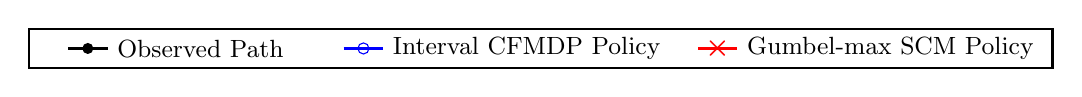
\begin{tikzpicture}[scale=1.0, every node/.style={scale=1.0}]
            \draw[thick, black] (-3, -0.25) rectangle (10, 0.25);
            %
            \draw[black, line width=1pt] (-2.5, 0.0) -- (-2,0.0);
            \fill[black] (-2.25,0.0) circle (2pt); %
            \node[right] at (-2,0.0) {\small Observed Path};
            
            %
            \draw[blue, line width=1pt] (1.0,0.0) -- (1.5,0.0);
            \node[draw=blue, circle, minimum size=4pt, inner sep=0pt] at (1.25,0.0) {}; %
            \node[right] at (1.5,0.0) {\small Interval CFMDP Policy};
            
            %
            \draw[red, line width=1pt] (5.5,0) -- (6,0);
            \node[red] at (5.75,0) {$\boldsymbol{\times}$}; %
            \node[right] at (6,0) {\small Gumbel-max SCM Policy};
        \end{tikzpicture}
    }\\
    %
    \subfigure[\footnotesize Lowest cumulative reward: Interval CFMDP ($312$), Gumbel-max SCM ($312$)]{%
        \resizebox{0.76\columnwidth}{!}{
             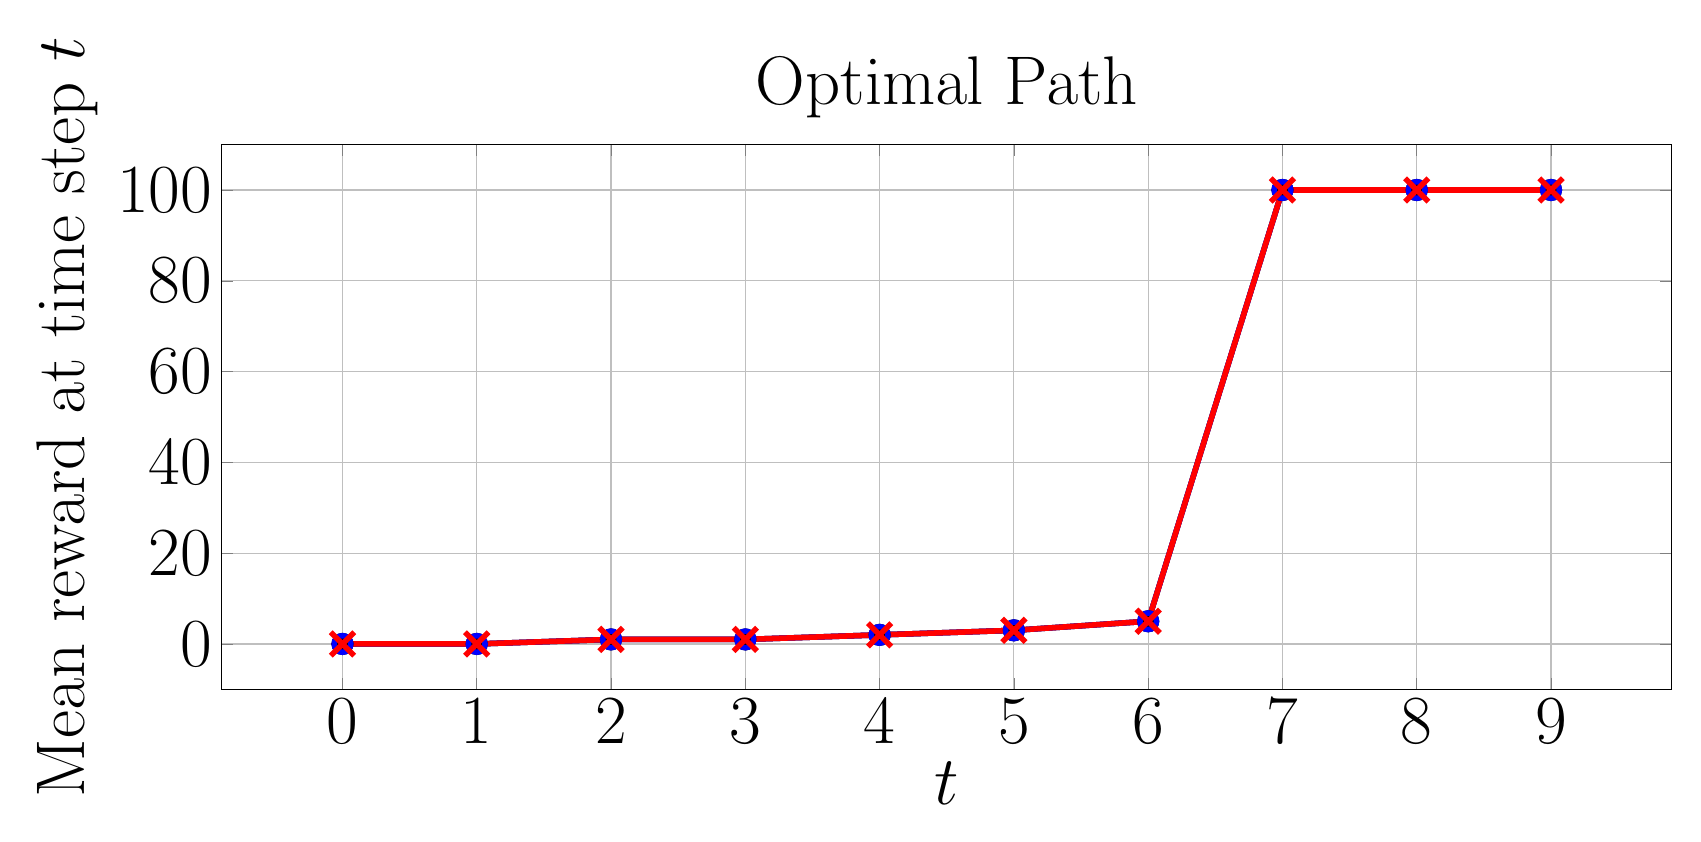
\begin{tikzpicture}
                \begin{axis}[
                    xlabel={$t$},
                    ylabel={Mean reward at time step $t$},
                    title={Optimal Path},
                    grid=both,
                    width=20cm, height=8.5cm,
                    every axis/.style={font=\Huge},
                    %
                ]
                \addplot[
                    color=black, %
                    mark=*, %
                    line width=2pt,
                    mark size=3pt,
                    error bars/.cd,
                    y dir=both, %
                    y explicit, %
                    error bar style={line width=1pt,solid},
                    error mark options={line width=1pt,mark size=4pt,rotate=90}
                ]
                coordinates {
                    (0, 0.0)  +- (0, 0.0)
                    (1, 0.0)  +- (0, 0.0) 
                    (2, 1.0)  +- (0, 0.0) 
                    (3, 1.0)  +- (0, 0.0)
                    (4, 2.0)  +- (0, 0.0)
                    (5, 3.0) +- (0, 0.0)
                    (6, 5.0) +- (0, 0.0)
                    (7, 100.0) +- (0, 0.0)
                    (8, 100.0) +- (0, 0.0)
                    (9, 100.0) +- (0, 0.0)
                };
                %
                \addplot[
                    color=blue, %
                    mark=o, %
                    line width=2pt,
                    mark size=3pt,
                    error bars/.cd,
                    y dir=both, %
                    y explicit, %
                    error bar style={line width=1pt,solid},
                    error mark options={line width=1pt,mark size=4pt,rotate=90}
                ]
                 coordinates {
                    (0, 0.0)  +- (0, 0.0)
                    (1, 0.0)  +- (0, 0.0) 
                    (2, 1.0)  +- (0, 0.0) 
                    (3, 1.0)  +- (0, 0.0)
                    (4, 2.0)  +- (0, 0.0)
                    (5, 3.0) +- (0, 0.0)
                    (6, 5.0) +- (0, 0.0)
                    (7, 100.0) +- (0, 0.0)
                    (8, 100.0) +- (0, 0.0)
                    (9, 100.0) +- (0, 0.0)
                };
                %
                \addplot[
                    color=red, %
                    mark=x, %
                    line width=2pt,
                    mark size=6pt,
                    error bars/.cd,
                    y dir=both, %
                    y explicit, %
                    error bar style={line width=1pt,solid},
                    error mark options={line width=1pt,mark size=4pt,rotate=90}
                ]
                coordinates {
                    (0, 0.0)  +- (0, 0.0)
                    (1, 0.0)  +- (0, 0.0) 
                    (2, 1.0)  +- (0, 0.0) 
                    (3, 1.0)  +- (0, 0.0)
                    (4, 2.0)  +- (0, 0.0)
                    (5, 3.0) +- (0, 0.0)
                    (6, 5.0) +- (0, 0.0)
                    (7, 100.0) +- (0, 0.0)
                    (8, 100.0) +- (0, 0.0)
                    (9, 100.0) +- (0, 0.0)
                };
                \end{axis}
            \end{tikzpicture}
         }
    }
    \hspace{1cm}
    \subfigure[\footnotesize Lowest cumulative reward: Interval CFMDP ($19$), Gumbel-max SCM ($-88$)]{%
         \resizebox{0.76\columnwidth}{!}{
            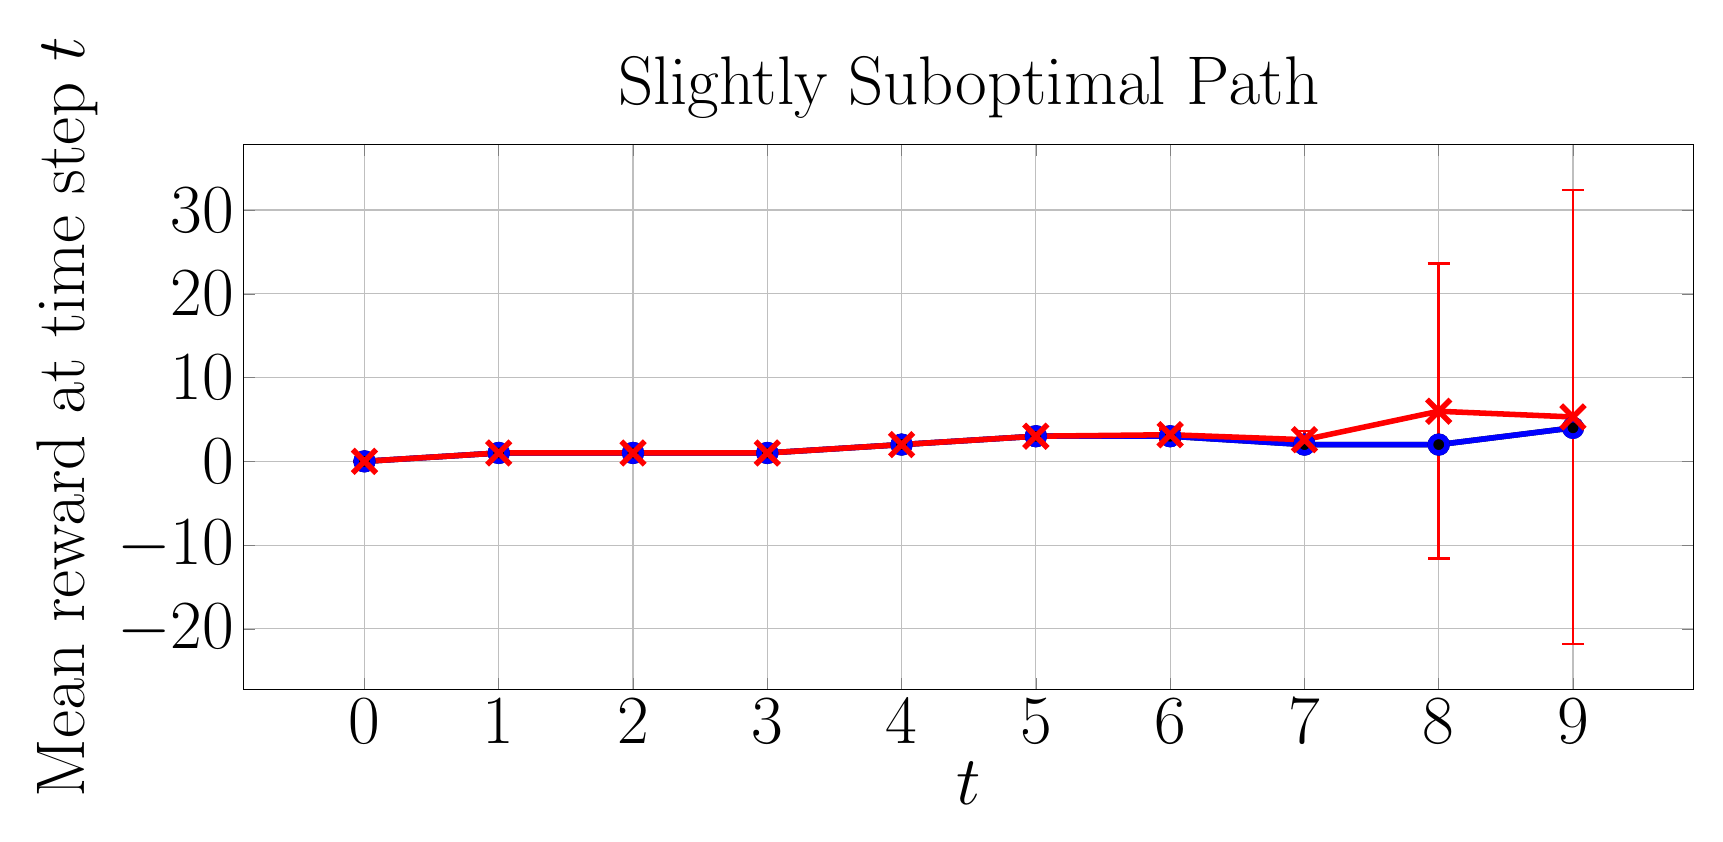
\begin{tikzpicture}
                \begin{axis}[
                    xlabel={$t$},
                    ylabel={Mean reward at time step $t$},
                    title={Slightly Suboptimal Path},
                    grid=both,
                    width=20cm, height=8.5cm,
                    every axis/.style={font=\Huge},
                    %
                ]
                \addplot[
                    color=black, %
                    mark=*, %
                    line width=2pt,
                    mark size=3pt,
                    error bars/.cd,
                    y dir=both, %
                    y explicit, %
                    error bar style={line width=1pt,solid},
                    error mark options={line width=1pt,mark size=4pt,rotate=90}
                ]
              coordinates {
                    (0, 0.0)  +- (0, 0.0)
                    (1, 1.0)  +- (0, 0.0) 
                    (2, 1.0)  +- (0, 0.0) 
                    (3, 1.0)  +- (0, 0.0)
                    (4, 2.0)  +- (0, 0.0)
                    (5, 3.0) +- (0, 0.0)
                    (6, 3.0) +- (0, 0.0)
                    (7, 2.0) +- (0, 0.0)
                    (8, 2.0) +- (0, 0.0)
                    (9, 4.0) +- (0, 0.0)
                };
                %
                \addplot[
                    color=blue, %
                    mark=o, %
                    line width=2pt,
                    mark size=3pt,
                    error bars/.cd,
                    y dir=both, %
                    y explicit, %
                    error bar style={line width=1pt,solid},
                    error mark options={line width=1pt,mark size=4pt,rotate=90}
                ]
              coordinates {
                    (0, 0.0)  +- (0, 0.0)
                    (1, 1.0)  +- (0, 0.0) 
                    (2, 1.0)  +- (0, 0.0) 
                    (3, 1.0)  +- (0, 0.0)
                    (4, 2.0)  +- (0, 0.0)
                    (5, 3.0) +- (0, 0.0)
                    (6, 3.0) +- (0, 0.0)
                    (7, 2.0) +- (0, 0.0)
                    (8, 2.0) +- (0, 0.0)
                    (9, 4.0) +- (0, 0.0)
                };
                %
                \addplot[
                    color=red, %
                    mark=x, %
                    line width=2pt,
                    mark size=6pt,
                    error bars/.cd,
                    y dir=both, %
                    y explicit, %
                    error bar style={line width=1pt,solid},
                    error mark options={line width=1pt,mark size=4pt,rotate=90}
                ]
                coordinates {
                    (0, 0.0)  +- (0, 0.0)
                    (1, 1.0)  +- (0, 0.0) 
                    (2, 1.0)  +- (0, 0.0) 
                    (3, 1.0)  +- (0, 0.0)
                    (4, 2.0)  += (0, 0.0)
                    (5, 3.0)  += (0, 0.0)
                    (6, 3.17847) += (0, 0.62606746) -= (0, 0.62606746)
                    (7, 2.5832885) += (0, 1.04598233) -= (0, 1.04598233)
                    (8, 5.978909) += (0, 17.60137623) -= (0, 17.60137623)
                    (9, 5.297059) += (0, 27.09227512) -= (0, 27.09227512)
                };
                \end{axis}
            \end{tikzpicture}
         }
    }\\[-1.5pt]
    \subfigure[\footnotesize Lowest cumulative reward: Interval CFMDP ($14$), Gumbel-max SCM ($-598$)]{%
         \resizebox{0.76\columnwidth}{!}{
             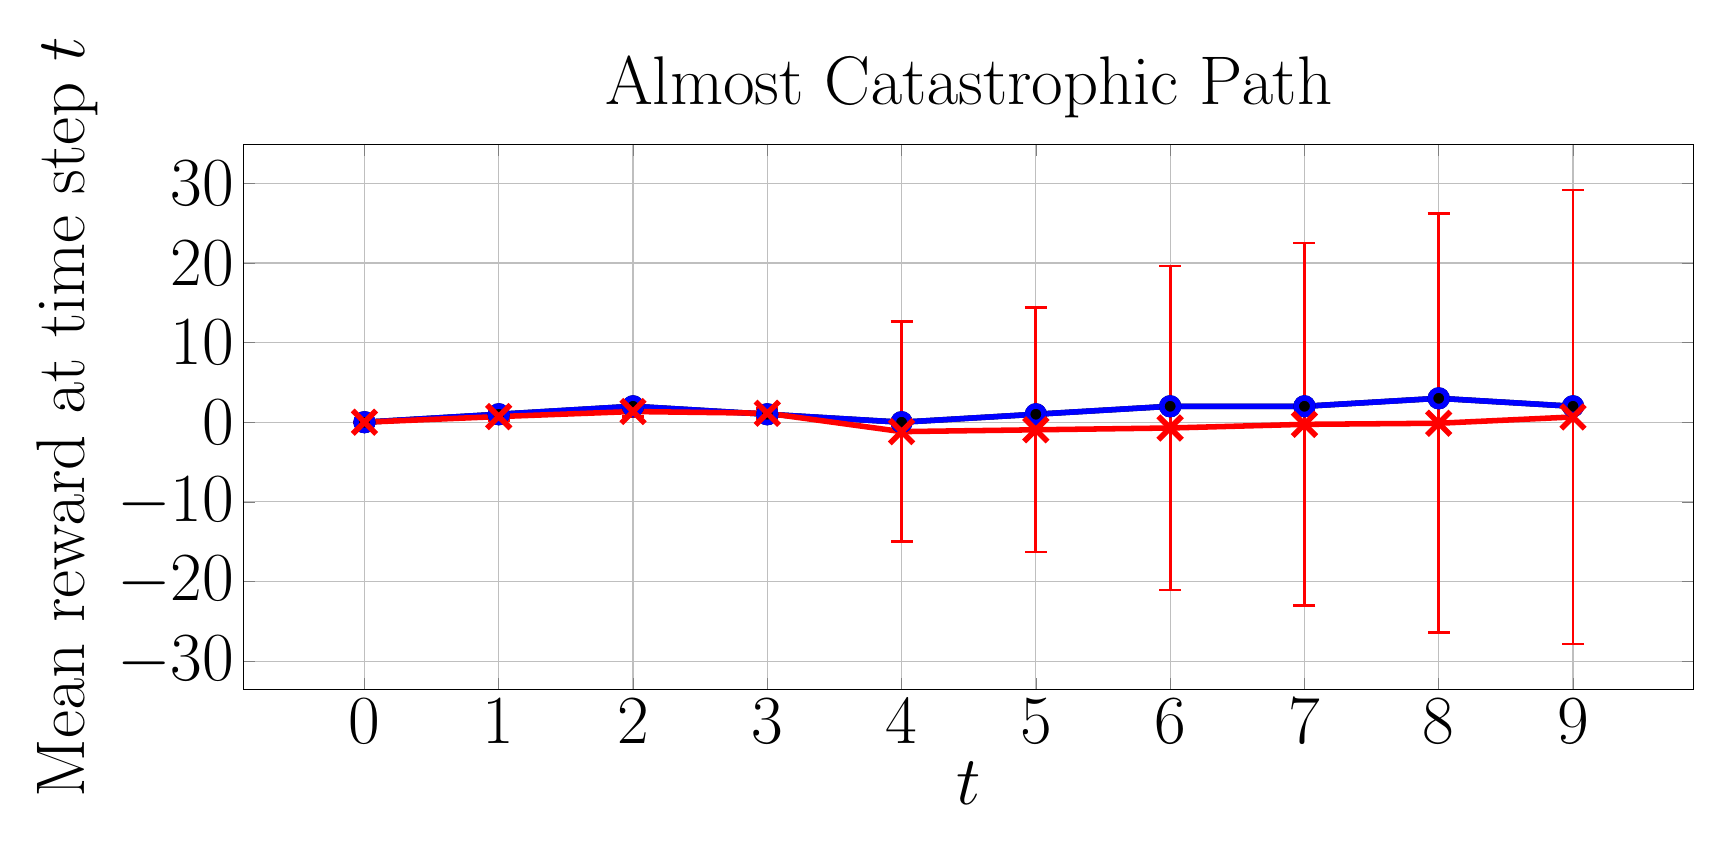
\begin{tikzpicture}
                \begin{axis}[
                    xlabel={$t$},
                    ylabel={Mean reward at time step $t$},
                    title={Almost Catastrophic Path},
                    grid=both,
                    width=20cm, height=8.5cm,
                    every axis/.style={font=\Huge},
                    %
                ]
                \addplot[
                    color=black, %
                    mark=*, %
                    line width=2pt,
                    mark size=3pt,
                    error bars/.cd,
                    y dir=both, %
                    y explicit, %
                    error bar style={line width=1pt,solid},
                    error mark options={line width=1pt,mark size=4pt,rotate=90}
                ]
                coordinates {
                    (0, 0.0)  +- (0, 0.0)
                    (1, 1.0)  +- (0, 0.0) 
                    (2, 2.0)  +- (0, 0.0) 
                    (3, 1.0)  +- (0, 0.0)
                    (4, 0.0)  +- (0, 0.0)
                    (5, 1.0) +- (0, 0.0)
                    (6, 2.0) +- (0, 0.0)
                    (7, 2.0) +- (0, 0.0)
                    (8, 3.0) +- (0, 0.0)
                    (9, 2.0) +- (0, 0.0)
                };
                %
                \addplot[
                    color=blue, %
                    mark=o, %
                    line width=2pt,
                    mark size=3pt,
                    error bars/.cd,
                    y dir=both, %
                    y explicit, %
                    error bar style={line width=1pt,solid},
                    error mark options={line width=1pt,mark size=4pt,rotate=90}
                ]
                coordinates {
                    (0, 0.0)  +- (0, 0.0)
                    (1, 1.0)  +- (0, 0.0) 
                    (2, 2.0)  +- (0, 0.0) 
                    (3, 1.0)  +- (0, 0.0)
                    (4, 0.0)  +- (0, 0.0)
                    (5, 1.0) +- (0, 0.0)
                    (6, 2.0) +- (0, 0.0)
                    (7, 2.0) +- (0, 0.0)
                    (8, 3.0) +- (0, 0.0)
                    (9, 2.0) +- (0, 0.0)
                };
                %
                \addplot[
                    color=red, %
                    mark=x, %
                    line width=2pt,
                    mark size=6pt,
                    error bars/.cd,
                    y dir=both, %
                    y explicit, %
                    error bar style={line width=1pt,solid},
                    error mark options={line width=1pt,mark size=4pt,rotate=90}
                ]
                coordinates {
                    (0, 0.0)  +- (0, 0.0)
                    (1, 0.7065655)  +- (0, 0.4553358) 
                    (2, 1.341673)  +- (0, 0.67091621) 
                    (3, 1.122926)  +- (0, 0.61281824)
                    (4, -1.1821935)  +- (0, 13.82444042)
                    (5, -0.952399)  +- (0, 15.35195457)
                    (6, -0.72672) +- (0, 20.33508414)
                    (7, -0.268983) +- (0, 22.77861454)
                    (8, -0.1310835) +- (0, 26.31013314)
                    (9, 0.65806) +- (0, 28.50670214)
                };
                %
            %
            %
            %
            %
            %
            %
            %
            %
            %
            %
            %
            %
            %
            %
            %
            %
            %
            %
                \end{axis}
            \end{tikzpicture}
         }
    }
    \hspace{1cm}
    \subfigure[\footnotesize Lowest cumulative reward: Interval CFMDP ($-698$), Gumbel-max SCM ($-698$)]{%
         \resizebox{0.76\columnwidth}{!}{
            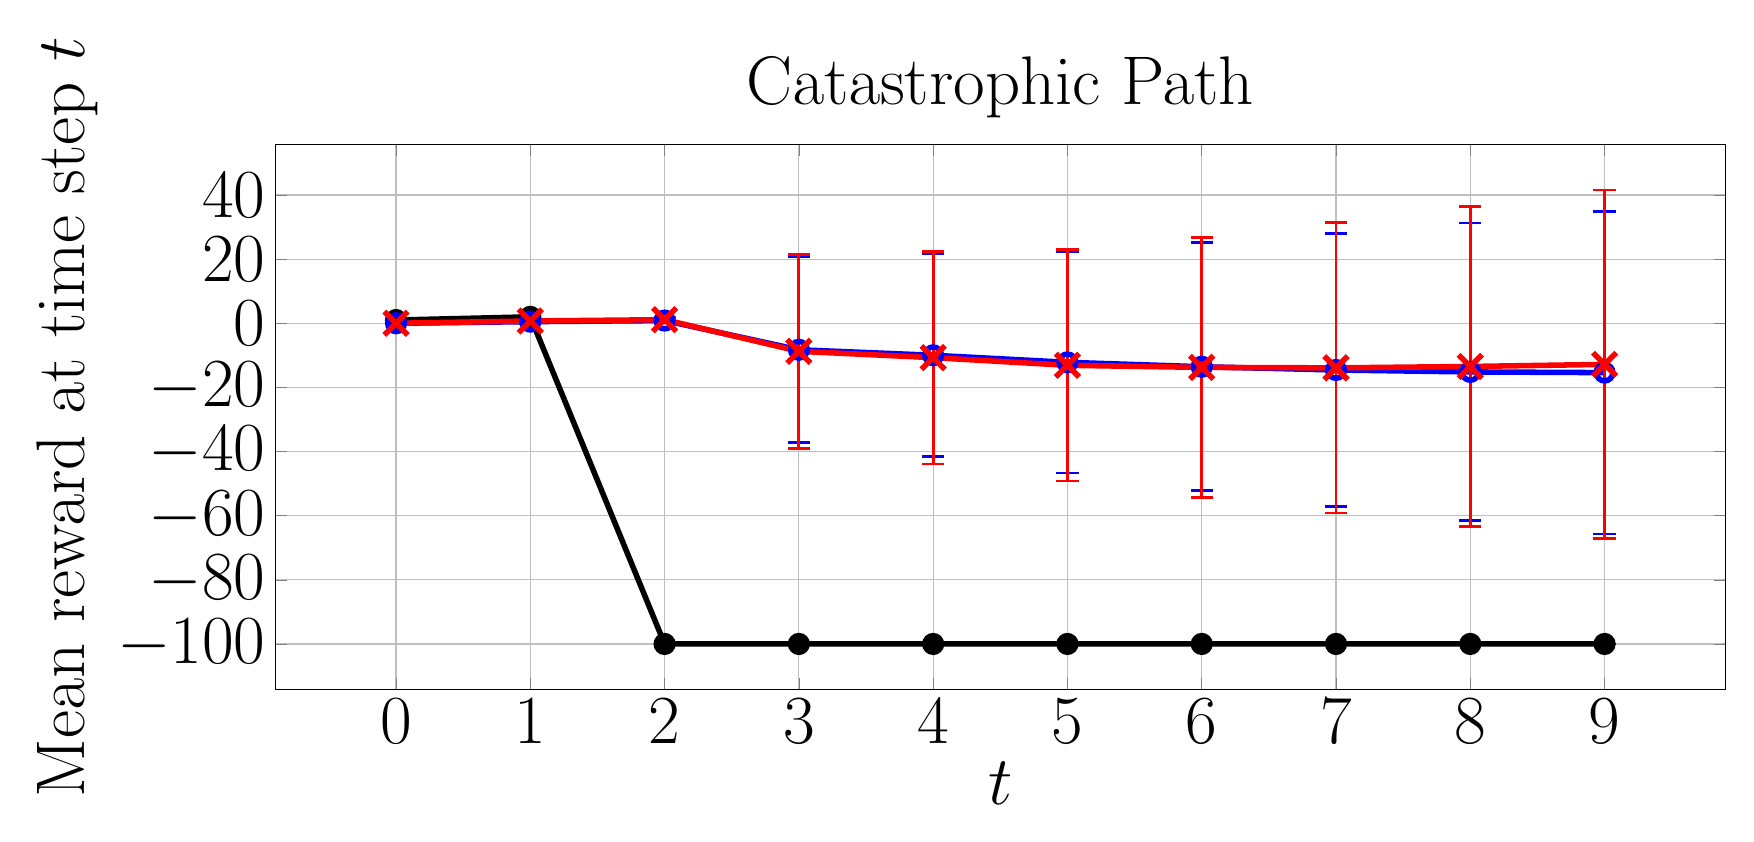
\begin{tikzpicture}
                \begin{axis}[
                    xlabel={$t$},
                    ylabel={Mean reward at time step $t$},
                    title={Catastrophic Path},
                    grid=both,
                    width=20cm, height=8.5cm,
                    every axis/.style={font=\Huge},
                    %
                ]
                \addplot[
                    color=black, %
                    mark=*, %
                    line width=2pt,
                    mark size=3pt,
                    error bars/.cd,
                    y dir=both, %
                    y explicit, %
                    error bar style={line width=1pt,solid},
                    error mark options={line width=1pt,mark size=4pt,rotate=90}
                ]
                coordinates {
                    (0, 1.0)  +- (0, 0.0)
                    (1, 2.0)  +- (0, 0.0) 
                    (2, -100.0)  +- (0, 0.0) 
                    (3, -100.0)  +- (0, 0.0)
                    (4, -100.0)  +- (0, 0.0)
                    (5, -100.0) +- (0, 0.0)
                    (6, -100.0) +- (0, 0.0)
                    (7, -100.0) +- (0, 0.0)
                    (8, -100.0) +- (0, 0.0)
                    (9, -100.0) +- (0, 0.0)
                };
                %
                \addplot[
                    color=blue, %
                    mark=o, %
                    line width=2pt,
                    mark size=3pt,
                    error bars/.cd,
                    y dir=both, %
                    y explicit, %
                    error bar style={line width=1pt,solid},
                    error mark options={line width=1pt,mark size=4pt,rotate=90}
                ]
                coordinates {
                    (0, 0.0)  +- (0, 0.0)
                    (1, 0.504814)  +- (0, 0.49997682) 
                    (2, 0.8439835)  +- (0, 0.76831917) 
                    (3, -8.2709165)  +- (0, 28.93656754)
                    (4, -9.981082)  +- (0, 31.66825363)
                    (5, -12.1776325) +- (0, 34.53463233)
                    (6, -13.556076) +- (0, 38.62845372)
                    (7, -14.574418) +- (0, 42.49603359)
                    (8, -15.1757075) +- (0, 46.41913968)
                    (9, -15.3900395) +- (0, 50.33563368)
                };
                %
                \addplot[
                    color=red, %
                    mark=x, %
                    line width=2pt,
                    mark size=6pt,
                    error bars/.cd,
                    y dir=both, %
                    y explicit, %
                    error bar style={line width=1pt,solid},
                    error mark options={line width=1pt,mark size=4pt,rotate=90}
                ]
                coordinates {
                    (0, 0.0)  +- (0, 0.0)
                    (1, 0.701873)  +- (0, 0.45743556) 
                    (2, 1.1227805)  +- (0, 0.73433129) 
                    (3, -8.7503255)  +- (0, 30.30257976)
                    (4, -10.722092)  +- (0, 33.17618589)
                    (5, -13.10721)  +- (0, 36.0648089)
                    (6, -13.7631645) +- (0, 40.56553451)
                    (7, -13.909043) +- (0, 45.23829402)
                    (8, -13.472517) +- (0, 49.96270296)
                    (9, -12.8278835) +- (0, 54.38618735)
                };
                %
            %
            %
            %
            %
            %
            %
            %
            %
            %
            %
            %
            %
            %
            %
            %
            %
            %
            %
                \end{axis}
            \end{tikzpicture}
         }
    }
    \caption{Average instant reward of CF paths induced by policies on GridWorld $p=0.4$.}
    \label{fig: reward p=0.4}
\end{figure*}

\subsection{Experimental Setup}
To compare policy performance, we measure the average rewards of counterfactual paths induced by our policy and the Gumbel-max policy by uniformly sampling $200$ counterfactual MDPs from the ICFMDP and generating $10,000$ counterfactual paths over each sampled CFMDP. \jl{Since the interval CFMDP depends on the observed path, we select $4$  paths of varying optimality to evaluate how the observed path impacts the performance of both policies: an optimal path, a slightly suboptimal path that could reach the optimal reward with a few changes, a catastrophic path that enters a catastrophic, terminal state with low reward, and an almost catastrophic path that was close to entering a catastrophic state.} When measuring the average probability bound widths and execution time needed to generate the ICFMDPs, we averaged over $20$ randomly generated observed paths
\footnote{Further training details are provided in Appendix \ref{app: training details}, and the code is provided at \href{https://github.com/ddv-lab/robust-cf-inference-in-MDPs}{https://github.com/ddv-lab/robust-cf-inference-in-MDPs}
%
%
.}.

\subsection{GridWorld}
\jl{The GridWorld MDP is a $4 \times 4$ grid where an agent must navigate from the top-left corner to the goal state in the bottom-right corner, avoiding a dangerous terminal state in the centre. At each time step, the agent can move up, down, left, or right, but there is a small probability (controlled by hyper-parameter $p$) of moving in an unintended direction. As the agent nears the goal, the reward for each state increases, culminating in a reward of $+100$ for reaching the goal. Entering the dangerous state results in a penalty of $-100$. We use two versions of GridWorld: a less stochastic version with $p=0.9$ (i.e., $90$\% chance of moving in the chosen direction) and a more stochastic version with $p=0.4$.}

\paragraph{GridWorld ($p=0.9$)}
When $p=0.9$, the counterfactual probability bounds are typically narrow (see Table \ref{tab:nonzero_probs} for average measurements). Consequently, as shown in Figure \ref{fig: reward p=0.9}, both policies are nearly identical and perform similarly well across the optimal, slightly suboptimal, and catastrophic paths.
%
However, for the almost catastrophic path, the interval CFMDP path is more conservative and follows the observed path more closely (as this is where the probability bounds are narrowest), which typically requires one additional step to reach the goal state than the Gumbel-max SCM policy.
%

\paragraph{GridWorld ($p=0.4$)}
\jl{When $p=0.4$, the GridWorld environment becomes more uncertain, increasing the risk of entering the dangerous state even if correct actions are chosen. Thus, as shown in Figure \ref{fig: reward p=0.4}, the interval CFMDP policy adopts a more conservative approach, avoiding deviation from the observed policy if it cannot guarantee higher counterfactual rewards (see the slightly suboptimal and almost catastrophic paths), whereas the Gumbel-max SCM is inconsistent: it can yield higher rewards, but also much lower rewards, reflected in the wide error bars.} For the catastrophic path, both policies must deviate from the observed path to achieve a higher reward and, in this case, perform similarly.
%
%
%
%
\subsection{Sepsis}
The Sepsis MDP \citep{oberst2019counterfactual} simulates trajectories of Sepsis patients. Each state consists of four vital signs (heart rate, blood pressure, oxygen concentration, and glucose levels), categorised as low, normal, or high.
and three treatments that can be toggled on/off at each time step (8 actions in total). Unlike \citet{oberst2019counterfactual}, we scale rewards based on the number of out-of-range vital signs, between $-1000$ (patient dies) and $1000$ (patient discharged). \jl{Like the GridWorld $p=0.4$ experiment, the Sepsis MDP is highly uncertain, as many states are equally likely to lead to optimal and poor outcomes. Thus, as shown in Figure \ref{fig: reward sepsis}, both policies follow the observed optimal and almost catastrophic paths to guarantee rewards are no worse than the observation.} However, improving the catastrophic path requires deviating from the observation. Here, the Gumbel-max SCM policy, on average, performs better than the interval CFMDP policy. But, since both policies have lower bounds clipped at $-1000$, neither policy reliably improves over the observation. In contrast, for the slightly suboptimal path, the interval CFMDP policy performs significantly better, shown by its higher lower bounds. 
Moreover, in these two cases, the worst-case counterfactual path generated by the interval CFMDP policy is better than that of the Gumbel-max SCM policy,
indicating its greater robustness.
%
\begin{figure*}
    \centering
     \resizebox{0.6\textwidth}{!}{
        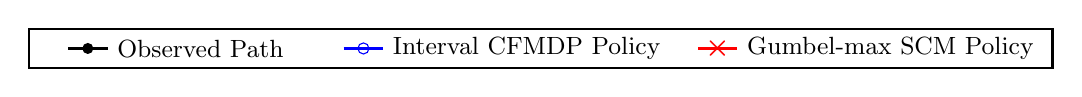
\begin{tikzpicture}[scale=1.0, every node/.style={scale=1.0}]
            \draw[thick, black] (-3, -0.25) rectangle (10, 0.25);
            %
            \draw[black, line width=1pt] (-2.5, 0.0) -- (-2,0.0);
            \fill[black] (-2.25,0.0) circle (2pt); %
            \node[right] at (-2,0.0) {\small Observed Path};
            
            %
            \draw[blue, line width=1pt] (1.0,0.0) -- (1.5,0.0);
            \node[draw=blue, circle, minimum size=4pt, inner sep=0pt] at (1.25,0.0) {}; %
            \node[right] at (1.5,0.0) {\small Interval CFMDP Policy};
            
            %
            \draw[red, line width=1pt] (5.5,0) -- (6,0);
            \node[red] at (5.75,0) {$\boldsymbol{\times}$}; %
            \node[right] at (6,0) {\small Gumbel-max SCM Policy};
        \end{tikzpicture}
    }\\
    \subfigure[\footnotesize Lowest cumulative reward: Interval CFMDP ($8000$), Gumbel-max SCM ($8000$)]{%
         \resizebox{0.76\columnwidth}{!}{
             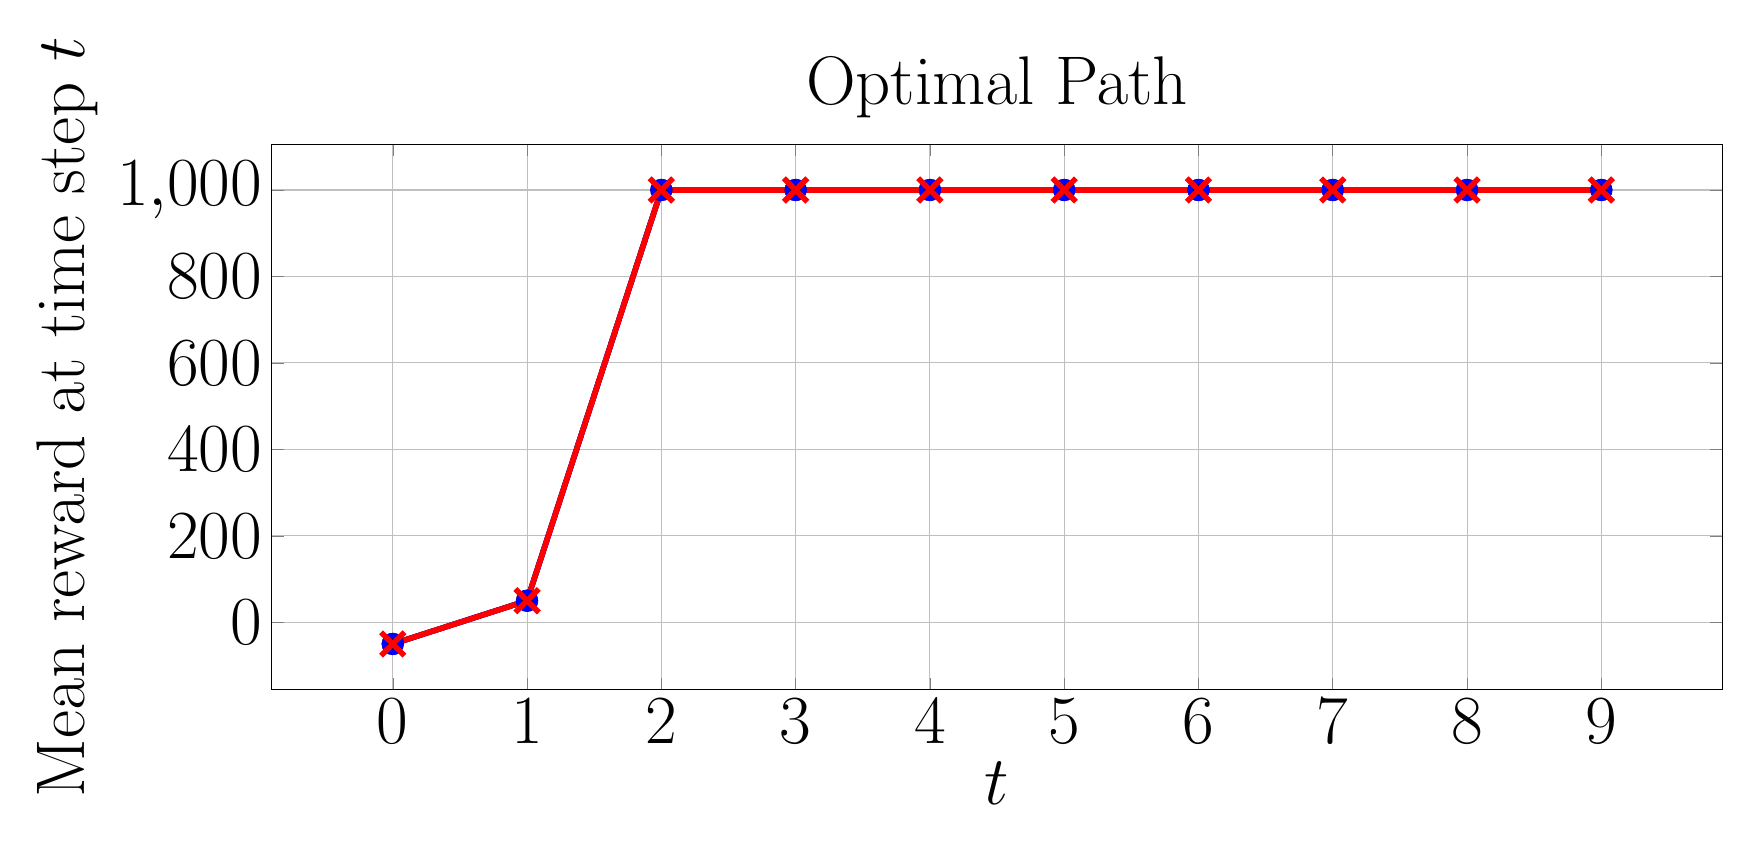
\begin{tikzpicture}
                \begin{axis}[
                    xlabel={$t$},
                    ylabel={Mean reward at time step $t$},
                    title={Optimal Path},
                    grid=both,
                    width=20cm, height=8.5cm,
                    every axis/.style={font=\Huge},
                    %
                ]
                \addplot[
                    color=black, %
                    mark=*, %
                    line width=2pt,
                    mark size=3pt,
                ]
                coordinates {
                    (0, -50.0)
                    (1, 50.0)
                    (2, 1000.0)
                    (3, 1000.0)
                    (4, 1000.0)
                    (5, 1000.0)
                    (6, 1000.0)
                    (7, 1000.0)
                    (8, 1000.0)
                    (9, 1000.0)
                };
                %
                \addplot[
                    color=blue, %
                    mark=o, %
                    line width=2pt,
                    mark size=3pt,
                    error bars/.cd,
                    y dir=both, %
                    y explicit, %
                    error bar style={line width=1pt,solid},
                    error mark options={line width=1pt,mark size=4pt,rotate=90}
                ]
                coordinates {
                    (0, -50.0)  +- (0, 0.0)
                    (1, 50.0)  +- (0, 0.0) 
                    (2, 1000.0)  +- (0, 0.0) 
                    (3, 1000.0)  +- (0, 0.0)
                    (4, 1000.0)  +- (0, 0.0)
                    (5, 1000.0) +- (0, 0.0)
                    (6, 1000.0) +- (0, 0.0)
                    (7, 1000.0) +- (0, 0.0)
                    (8, 1000.0) +- (0, 0.0)
                    (9, 1000.0) +- (0, 0.0)
                };
                %
                \addplot[
                    color=red, %
                    mark=x, %
                    line width=2pt,
                    mark size=6pt,
                    error bars/.cd,
                    y dir=both, %
                    y explicit, %
                    error bar style={line width=1pt,solid},
                    error mark options={line width=1pt,mark size=4pt,rotate=90}
                ]
                coordinates {
                    (0, -50.0)  +- (0, 0.0)
                    (1, 50.0)  +- (0, 0.0) 
                    (2, 1000.0)  +- (0, 0.0) 
                    (3, 1000.0)  +- (0, 0.0)
                    (4, 1000.0)  +- (0, 0.0)
                    (5, 1000.0) +- (0, 0.0)
                    (6, 1000.0) +- (0, 0.0)
                    (7, 1000.0) +- (0, 0.0)
                    (8, 1000.0) +- (0, 0.0)
                    (9, 1000.0) +- (0, 0.0)
                };
                %
                \end{axis}
            \end{tikzpicture}
         }
    }
    \hspace{1cm}
    \subfigure[\footnotesize Lowest cumulative reward: Interval CFMDP ($-5980$), Gumbel-max SCM ($-8000$)]{%
         \resizebox{0.76\columnwidth}{!}{
            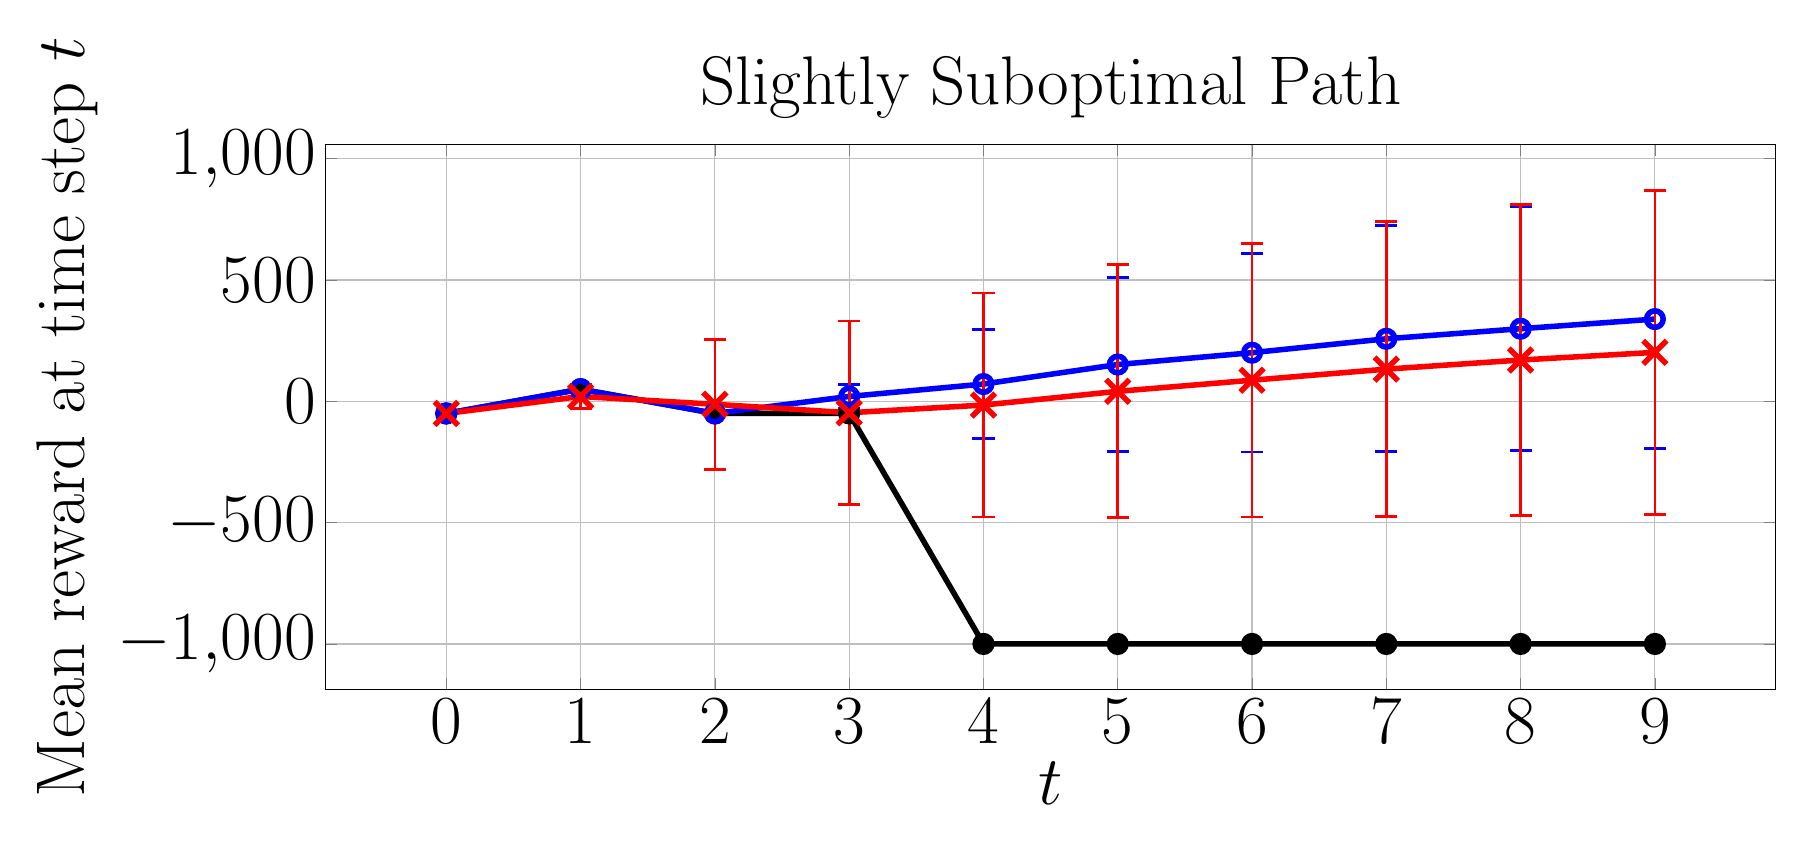
\begin{tikzpicture}
                \begin{axis}[
                    xlabel={$t$},
                    ylabel={Mean reward at time step $t$},
                    title={Slightly Suboptimal Path},
                    grid=both,
                    width=20cm, height=8.5cm,
                    every axis/.style={font=\Huge},
                    %
                ]
               \addplot[
                    color=black, %
                    mark=*, %
                    line width=2pt,
                    mark size=3pt,
                ]
                coordinates {
                    (0, -50.0)
                    (1, 50.0)
                    (2, -50.0)
                    (3, -50.0)
                    (4, -1000.0)
                    (5, -1000.0)
                    (6, -1000.0)
                    (7, -1000.0)
                    (8, -1000.0)
                    (9, -1000.0)
                };
                %
                \addplot[
                    color=blue, %
                    mark=o, %
                    line width=2pt,
                    mark size=3pt,
                    error bars/.cd,
                    y dir=both, %
                    y explicit, %
                    error bar style={line width=1pt,solid},
                    error mark options={line width=1pt,mark size=4pt,rotate=90}
                ]
                coordinates {
                    (0, -50.0)  +- (0, 0.0)
                    (1, 50.0)  +- (0, 0.0) 
                    (2, -50.0)  +- (0, 0.0) 
                    (3, 20.0631)  +- (0, 49.97539413)
                    (4, 71.206585)  +- (0, 226.02033693)
                    (5, 151.60797) +- (0, 359.23292559)
                    (6, 200.40593) +- (0, 408.86185176)
                    (7, 257.77948) +- (0, 466.10372804)
                    (8, 299.237465) +- (0, 501.82579506)
                    (9, 338.9129) +- (0, 532.06124996)
                };
                %
                \addplot[
                    color=red, %
                    mark=x, %
                    line width=2pt,
                    mark size=6pt,
                    error bars/.cd,
                    y dir=both, %
                    y explicit, %
                    error bar style={line width=1pt,solid},
                    error mark options={line width=1pt,mark size=4pt,rotate=90}
                ]
                coordinates {
                    (0, -50.0)  +- (0, 0.0)
                    (1, 20.00736)  +- (0, 49.99786741) 
                    (2, -12.282865)  +- (0, 267.598755) 
                    (3, -47.125995)  +- (0, 378.41755832)
                    (4, -15.381965)  +- (0, 461.77616558)
                    (5, 41.15459) +- (0, 521.53189262)
                    (6, 87.01595) +- (0, 564.22243126 )
                    (7, 132.62376) +- (0, 607.31338037)
                    (8, 170.168145) +- (0, 641.48013693)
                    (9, 201.813135) +- (0, 667.29441777)
                };
                %
                %
                %
                %
                %
                %
                %
                %
                %
                %
                %
                %
                %
                %
                %
                %
                %
                %
                %
                \end{axis}
            \end{tikzpicture}
         }
    }\\[-1.5pt]
    \subfigure[\footnotesize Lowest cumulative reward: Interval CFMDP ($100$), Gumbel-max SCM ($100$)]{%
         \resizebox{0.76\columnwidth}{!}{
             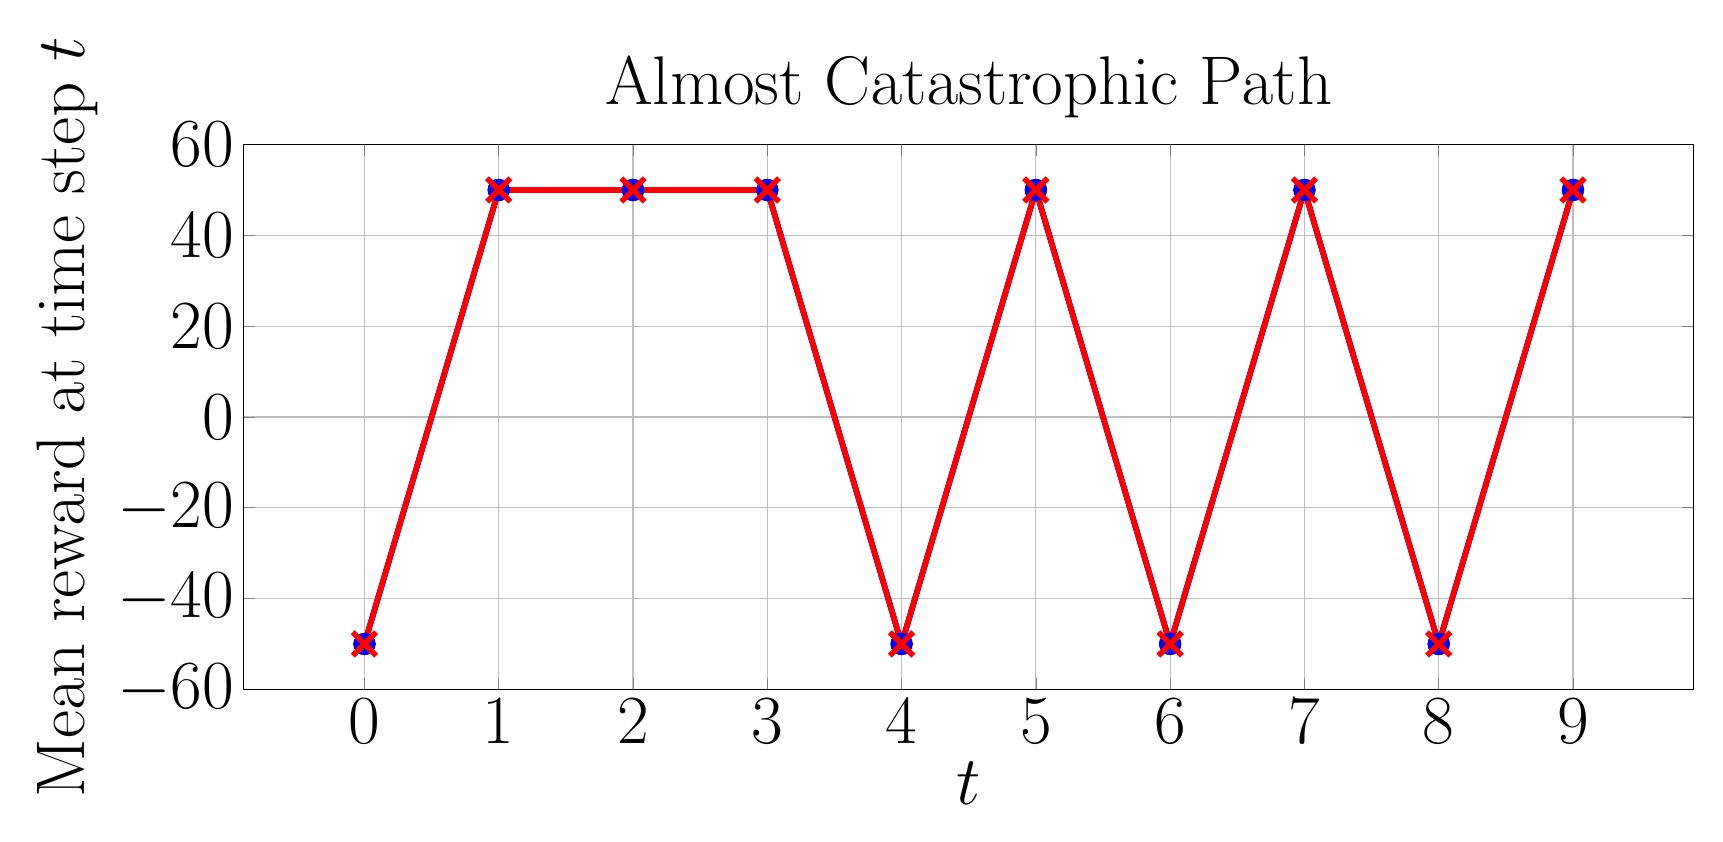
\begin{tikzpicture}
                \begin{axis}[
                    xlabel={$t$},
                    ylabel={Mean reward at time step $t$},
                    title={Almost Catastrophic Path},
                    grid=both,
                    every axis/.style={font=\Huge},
                    width=20cm, height=8.5cm,
                    %
                ]
               \addplot[
                    color=black, %
                    mark=*, %
                    line width=2pt,
                    mark size=3pt,
                ]
                coordinates {
                    (0, -50.0)
                    (1, 50.0)
                    (2, 50.0)
                    (3, 50.0)
                    (4, -50.0)
                    (5, 50.0)
                    (6, -50.0)
                    (7, 50.0)
                    (8, -50.0)
                    (9, 50.0)
                };
                %
                %
                \addplot[
                    color=blue, %
                    mark=o, %
                    line width=2pt,
                    mark size=3pt,
                    error bars/.cd,
                    y dir=both, %
                    y explicit, %
                    error bar style={line width=1pt,solid},
                    error mark options={line width=1pt,mark size=4pt,rotate=90}
                ]
                coordinates {
                    (0, -50.0)  +- (0, 0.0)
                    (1, 50.0)  +- (0, 0.0) 
                    (2, 50.0)  +- (0, 0.0) 
                    (3, 50.0)  +- (0, 0.0)
                    (4, -50.0)  +- (0, 0.0)
                    (5, 50.0) +- (0, 0.0)
                    (6, -50.0) +- (0, 0.0)
                    (7, 50.0) +- (0, 0.0)
                    (8, -50.0) +- (0, 0.0)
                    (9, 50.0) +- (0, 0.0)
                };
                %
                \addplot[
                    color=red, %
                    mark=x, %
                    line width=2pt,
                    mark size=6pt,
                    error bars/.cd,
                    y dir=both, %
                    y explicit, %
                    error bar style={line width=1pt,solid},
                    error mark options={line width=1pt,mark size=4pt,rotate=90}
                ]
                coordinates {
                    (0, -50.0)  +- (0, 0.0)
                    (1, 50.0)  +- (0, 0.0) 
                    (2, 50.0)  +- (0, 0.0) 
                    (3, 50.0)  +- (0, 0.0)
                    (4, -50.0)  +- (0, 0.0)
                    (5, 50.0) +- (0, 0.0)
                    (6, -50.0) +- (0, 0.0)
                    (7, 50.0) +- (0, 0.0)
                    (8, -50.0) +- (0, 0.0)
                    (9, 50.0) +- (0, 0.0)
                };
                %
                %
                %
                %
                %
                %
                %
                %
                %
                %
                %
                %
                %
                %
                %
                %
                %
                %
                %
                \end{axis}
            \end{tikzpicture}
         }
    }
    \hspace{1cm}
    \subfigure[\footnotesize Lowest cumulative reward: Interval CFMDP ($-7150$), Gumbel-max SCM ($-9050$)]{%
         \resizebox{0.76\columnwidth}{!}{
            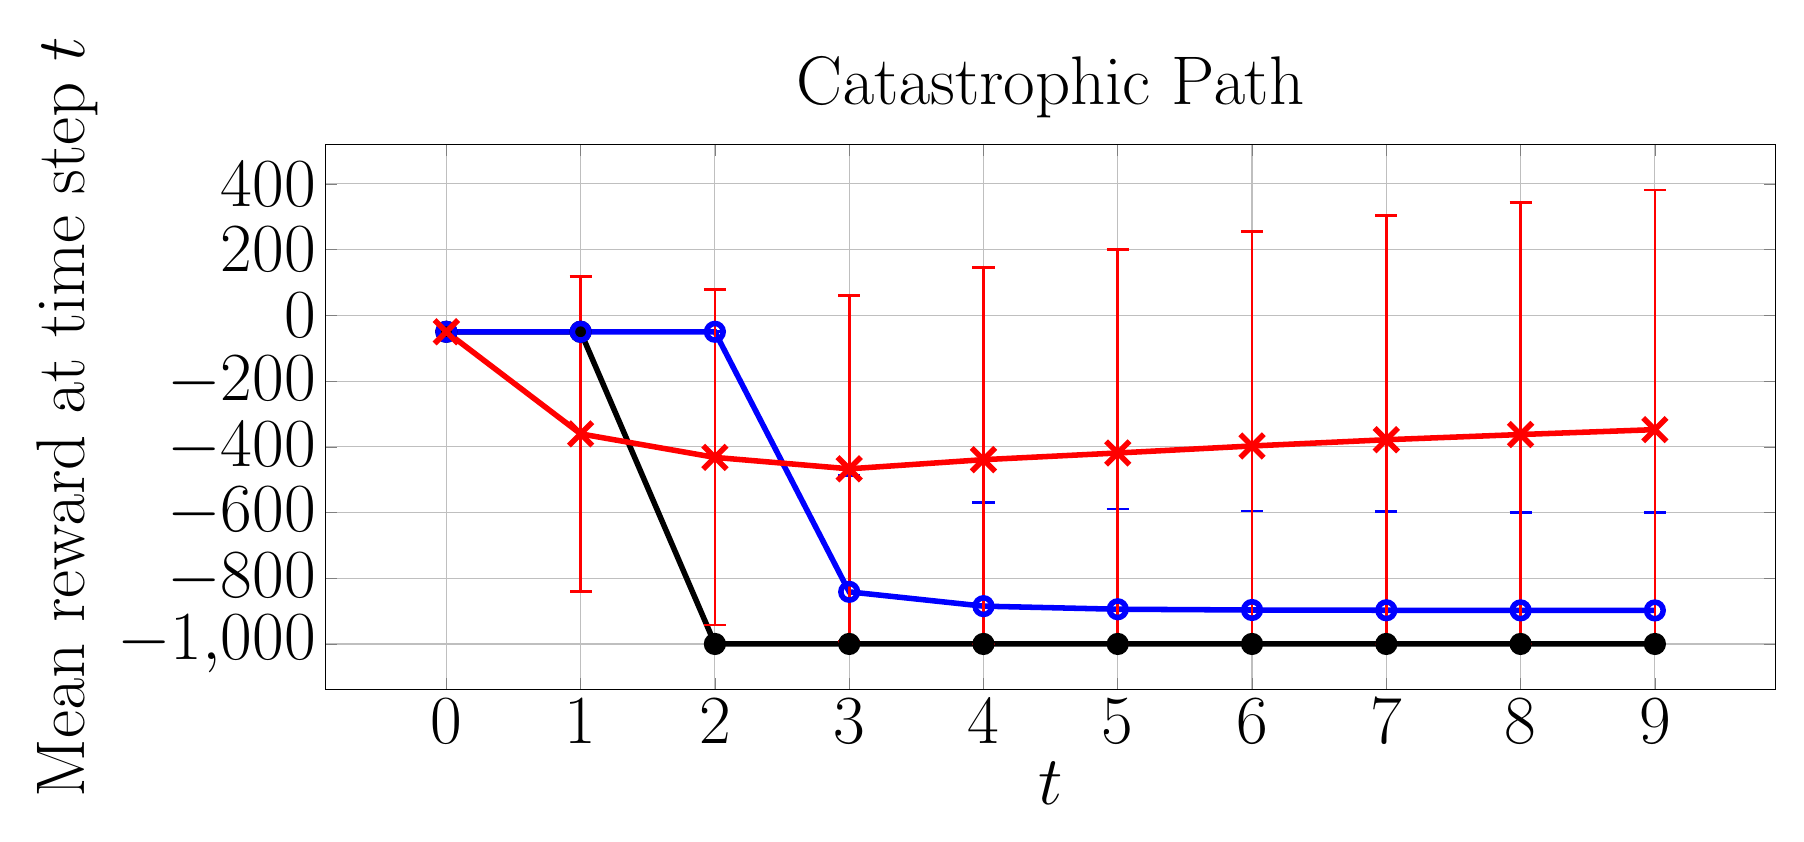
\begin{tikzpicture}
                \begin{axis}[
                    xlabel={$t$},
                    ylabel={Mean reward at time step $t$},
                    title={Catastrophic Path},
                    grid=both,
                    width=20cm, height=8.5cm,
                    every axis/.style={font=\Huge},
                    %
                ]
               \addplot[
                    color=black, %
                    mark=*, %
                    line width=2pt,
                    mark size=3pt,
                ]
                coordinates {
                    (0, -50.0)
                    (1, -50.0)
                    (2, -1000.0)
                    (3, -1000.0)
                    (4, -1000.0)
                    (5, -1000.0)
                    (6, -1000.0)
                    (7, -1000.0)
                    (8, -1000.0)
                    (9, -1000.0)
                };
                %
                %
                \addplot[
                    color=blue, %
                    mark=o, %
                    line width=2pt,
                    mark size=3pt,
                    error bars/.cd,
                    y dir=both, %
                    y explicit, %
                    error bar style={line width=1pt,solid},
                    error mark options={line width=1pt,mark size=4pt,rotate=90}
                ]
                coordinates {
                    (0, -50.0)  +- (0, 0.0)
                    (1, -50.0)  +- (0, 0.0) 
                    (2, -50.0)  +- (0, 0.0) 
                    (3, -841.440725)  += (0, 354.24605512) -= (0, 158.559275)
                    (4, -884.98225)  += (0, 315.37519669) -= (0, 115.01775)
                    (5, -894.330425) += (0, 304.88572805) -= (0, 105.669575)
                    (6, -896.696175) += (0, 301.19954514) -= (0, 103.303825)
                    (7, -897.4635) += (0, 299.61791279) -= (0, 102.5365)
                    (8, -897.77595) += (0, 298.80392585) -= (0, 102.22405)
                    (9, -897.942975) += (0, 298.32920557) -= (0, 102.057025)
                };
                %
                \addplot[
                    color=red, %
                    mark=x, %
                    line width=2pt,
                    mark size=6pt,
                    error bars/.cd,
                    y dir=both, %
                    y explicit, %
                    error bar style={line width=1pt,solid},
                    error mark options={line width=1pt,mark size=4pt,rotate=90}
                ]
            coordinates {
                    (0, -50.0)  +- (0, 0.0)
                    (1, -360.675265)  +- (0, 479.39812699) 
                    (2, -432.27629)  +- (0, 510.38620897) 
                    (3, -467.029545)  += (0, 526.36009628) -= (0, 526.36009628)
                    (4, -439.17429)  += (0, 583.96638919) -= (0, 560.82571)
                    (5, -418.82704) += (0, 618.43027478) -= (0, 581.17296)
                    (6, -397.464895) += (0, 652.67322574) -= (0, 602.535105)
                    (7, -378.49052) += (0, 682.85407033) -= (0, 621.50948)
                    (8, -362.654195) += (0, 707.01412023) -= (0, 637.345805)
                    (9, -347.737935) += (0, 729.29076479) -= (0, 652.262065)
                };
                %
                %
                %
                %
                %
                %
                %
                %
                %
                %
                %
                %
                %
                %
                %
                %
                %
                %
                %
                \end{axis}
            \end{tikzpicture}
         }
    }
    \caption{Average instant reward of CF paths induced by policies on Sepsis.}
    \label{fig: reward sepsis}
\end{figure*}

%
%
%
\subsection{Interval CFMDP Bounds}
%
%
Table \ref{tab:nonzero_probs} presents the mean counterfactual probability bound widths (excluding transitions where the upper bound is $0$) for each MDP, averaged over 20 observed paths. We compare the bounds under counterfactual stability (CS) and monotonicity (M) assumptions, CS alone, and no assumptions. This shows that the assumptions marginally reduce the bound widths, indicating the assumptions tighten the bounds without excluding too many causal models, as intended.
\renewcommand{\arraystretch}{1}

\begin{table}
\centering
\caption{Mean width of counterfactual probability bounds}
\resizebox{0.8\columnwidth}{!}{%
\begin{tabular}{|c|c|c|c|}
\hline
\multirow{2}{*}{\textbf{Environment}} & \multicolumn{3}{c|}{\textbf{Assumptions}} \\ \cline{2-4}
 & \textbf{CS + M} & \textbf{CS} & \textbf{None\tablefootnote{\jl{Equivalent to \citet{li2024probabilities}'s bounds (see Section \ref{sec: equivalence with Li}).}}} \\ \hline
\textbf{GridWorld} ($p=0.9$) & 0.0817 & 0.0977 & 0.100 \\ \hline
\textbf{GridWorld} ($p=0.4$) & 0.552  & 0.638  & 0.646 \\ \hline
\textbf{Sepsis} & 0.138 & 0.140 & 0.140 \\ \hline
\end{tabular}
}
\label{tab:nonzero_probs}
\end{table}


\subsection{Execution Times}
Table \ref{tab: times} compares the average time needed to generate the interval CFMDP vs.\ the Gumbel-max SCM CFMDP for 20 observations.
The GridWorld algorithms were run single-threaded, while the Sepsis experiments were run in parallel.
Generating the interval CFMDP is significantly faster as it uses exact analytical bounds, whereas the Gumbel-max CFMDP requires sampling from the Gumbel distribution to estimate counterfactual transition probabilities. \jl{Since constructing the counterfactual MDP models is the main bottleneck in both approaches, ours is more efficient overall and suitable for larger MDPs.}
\begin{table}
\centering
\caption{Mean execution time to generate CFMDPs}
\resizebox{0.99\columnwidth}{!}{%
\begin{tabular}{|c|c|c|}
\hline
\multirow{2}{*}{\textbf{Environment}} & \multicolumn{2}{c|}{\textbf{Mean Execution Time (s)}} \\ \cline{2-3} 
                                      & \textbf{Interval CFMDP} & \textbf{Gumbel-max CFMDP} \\ \hline
\textbf{GridWorld ($p=0.9$) }                  & 0.261                   & 56.1                      \\ \hline
\textbf{GridWorld ($p=0.4$)  }                 & 0.336                   & 54.5                      \\ \hline
\textbf{Sepsis}                                 & 688                     & 2940                      \\ \hline
\end{tabular}%
}
\label{tab: times}
\end{table}

\section{Conclusion}
In this work, we propose a simple yet effective approach, called SMILE, for graph few-shot learning with fewer tasks. Specifically, we introduce a novel dual-level mixup strategy, including within-task and across-task mixup, for enriching the diversity of nodes within each task and the diversity of tasks. Also, we incorporate the degree-based prior information to learn expressive node embeddings. Theoretically, we prove that SMILE effectively enhances the model's generalization performance. Empirically, we conduct extensive experiments on multiple benchmarks and the results suggest that SMILE significantly outperforms other baselines, including both in-domain and cross-domain few-shot settings.

\section{Acknowledgements}
This research was supported by the Quantum Internet Alliance through the European Union's Horizon 2020 program under grant agreement No. 820445 
and from the Horizon Europe program grant agreement No. 101080128.
We furthermore acknowledge support from NWO (including a VICI grant).

We thank 
Przemysław Pawełczak,
Michele Amoretti,
Anabel Ovide,
Thomas Beauchamp,
Álvaro Gomez Iniesta,
Ingmar te Raa,
Diego Rivera and
Francisco Silva
for useful discussions and feedback on (early) drafts.


\section{Data availability}
The implementation of Qoala as a simulator can be found online~\cite{qoala2023simulator}.
The code and data supporting the evaluation can be found at~\cite{evaluation-data}.

\bibliographystyle{unsrt}
\bibliography{qoala-paper}


% \clearpage
\appendices

\onecolumn

\section*{Appendix}
Appendix containing additional information for the paper \textbf{Qoala: an Application Execution Environment for Quantum Internet Nodes}.
This Appendix is structured as follows.
\begin{itemize}
\item \cref{app:program_structure} provides details of the \textbf{Qoala program format}.
\item \cref{app:runtime_environment} provides details of the \textbf{Qoala runtime environment}.
\item In \cref{app:scheduling_execution}, our \textbf{scheduler implementation} (\cref{sec:implementation}) is explained more in-depth.
\item \cref{app:simulator} gives an overview of our \textbf{simulator implementation}.
\item In \cref{app:evaluation} we elaborate on our \textbf{evaluations}.
\end{itemize}


\section{Program structure}
\label{app:program_structure}
This section provides details about the structure and contents of Qoala programs as described in \cref{sec:program_structure}.


\subsection{Program representation and components}
A Qoala program is represented in human-readable text format.
This allows one to directly write Qoala programs, although our vision is that programmers write their code in a higher-level language, and that a compiler translates this into a Qoala program.

In the main text, some parts of example programs were omitted for brevity.
In \cref{fig:app:example_full_program} we show an example of a full Qoala program.

A Qoala program encompasses both classical and quantum code.
These different code segments are put into different sections in the program.
The host section contains QoalaHost code which is to be run on the CPS.
The NetQASM section contains local routines (containing NetQASM instructions) which are meant to be run on the QPS.
The request section contains specifications of requests for remote entanglement generation, to be handled by the QPS.
Furthermore, there is a meta section which defines global information about the program.
Each of these sections is explained in more detail below.

In all of the sections in a Qoala program, values may be replaced by a \textbf{template}.
A template represents a value that is not defined for the program, but is filled in at program instantiation. For example, a QKD program might have a request object in its request section containing the entry \texttt{num\_pairs: {N}}, where \texttt{{N}} is a template. This construction allows one to instantiate the same program with different values for \texttt{N}, and it is hence not needed to define separate programs for each different number of pairs to generate in the QKD program.

\subsection{Program Meta}
Program metadata contains:

\begin{itemize}
    \item \textbf{Name}: The name of this program.
    \item \textbf{Parameters}: Global arguments to this program. These arguments may be used as templates (see above) in the program. Examples may be the name of a remote node, or the number of EPR pairs to generate.
    \item \textbf{Classical Sockets}: A mapping from IDs to remote node names. The IDs are local identifiers that can be used by Host code to distinguish different classical sockets.
    \item \textbf{EPR Sockets}: A mapping from IDs to remote node names. The IDs are local identifiers that can be used by Host code to distinguish different EPR sockets.
\end{itemize}




\begin{figure*}[htbp]
    \centering
    \begin{minipage}{\textwidth}
        \lstinputlisting[language=qoala, caption={}]{sections/appendix/full_program.iqoala}
    \end{minipage}
    \caption{Example Qoala program which creates an EPR pair with remote program Alice, measures the local qubit, and returns the classical outcome value.
    \textit{Meta section.} The meta section defines the name of this program, the global arguments (input values, in this case: the node ID of the Alice program),
    the classical sockets used (mapping local socket ID to the name of the remote node, and the EPR sockets used (also mapping local socket ID to remote node names)).
    \textit{Host section.} This example host section consists of three blocks (\texttt{b1, b2, b3}). \texttt{b1} calls request routine \texttt{req} (no result values).
    \texttt{b2} calls local routine \texttt{post\_epr}, resulting in a classical vector with one value (\texttt{m0}).
    \texttt{b3} returns \texttt{m0} as the result of this program.
    \textit{Local routines section.} Consists of a single local routine called \texttt{post\_epr}.
    It requires the virtual qubit (see \cref{app:runtime_environment}) with ID 0 to be allocated, and acts on this qubit.
    Upon finishing the local routine, this qubit is not in use anymore (the \texttt{keeps} entry is empty).
    The NetQASM code represents measuring the qubit, and then storing the result (in register \texttt{M0}) to the \texttt{@output} array (see \cref{app:runtime_environment}), which is in shared memory and can be accessed by host code by the name \texttt{m0}.
    \textit{Request routines section.} Consists of a single request routine called \texttt{req}.
    It represents a request to the network stack for generating a single entangled pair (\texttt{num\_pairs} is 1), which is kept in memory (\texttt{typ: create\_keep}; not measured immediately).
    This program acts as a `receiver' for entanglement generation (\texttt{role} attribute), which breaks symmetry in the entanglement generation process (the remote Alice program will have \texttt{role: sender}). Symmetry breaking is needed for the network stack to organize the entanglement generation.
    No callbacks are used, and all qubits (in this case: one) are stored in virtual qubit 0.
    }
    \label{fig:app:example_full_program}
\end{figure*}



\subsection{Host section}
The host section contains code the be executed by the CPS.
It consists of both local processing (like calculation and conditional logic), and
communication (sending and receiving classical messages to and from other nodes in the network).

The language in which host code is represented is called QoalaHost.
This is a low-level instruction set with well-defined semantics and types,
and is meant to be executed by a virtual machine or interpreter.
One can also imagine QoalaHost code to be translated (either ahead-of-time or at just-in-time) to native CPS code, such as x86 or ARM. However, for the sake of simplicity and of implementation independence, we treat here only the QoalaHost language and its semantics itself.

The QoalaHost (QH) language was designed to resemble intermediate representations as found in LLVM~\cite{lattner2004llvm} and MLIR~\cite{lattner2021mlir},
such that integration with future compilers is accessible.
Specifically, one may imagine a compiler that uses MLIR for its intermediate representation (IR).
When this compiler then produces the host code of the program, the translation of its own IR to QoalaHost code should be straightforward.

\textbf{Blocks.} 
The Host section consists of a list of blocks.
A block consists of a block metadata and a list of QH instructions.

The block metadata contains the following entries:
\begin{itemize}
\item \textbf{Name}: The name of this block. Host code can refer to this name in QH branch instructions.
\item \textbf{Type}: one of CL, CC, QL or QC (see below).
\item \textbf{Deadlines}: Deadlines relative to other blocks.
The deadlines are specified in terms of EHI arguments. Upon program instantiation, concrete values are filled in based on the actual EHI value.
\item \textbf{Time hints}: Duration estimate of executing the block.
The estimates are specified in terms of EHI arguments. Upon program instantiation, concrete values are filled in based on the actual EHI value.
\end{itemize}


\subsection{Block types}
Blocks are categorized into the following four types:
\begin{itemize}
\item \textbf{CL}: Classical Local. The block contains only instructions that are classical, local and only involve the CPS
\item \textbf{CC}: Classical Communication. CPS-only instructions, but starts with a `receive message` instruction.
\item \textbf{QL}: Quantum Local. The block contains calls to local routines.
\item \textbf{QC}: Quantum Communication. The block contains calls to request routines.
\end{itemize}


\textbf{QoalaHost Language.}
The QH Language describes a fixed set of QH instructions as well as QH Variable types.
Host code is represented as blocks containing QH instructions.
These instructions may be directly interpreted by a processor or OS.

All basic values are 32-bit signed integers (i32) or floating point values (f32).
A variable in Host code can either be
\begin{itemize}
\item singleton variable, holding one basic value. Has a single name. E.g. \texttt{x}
\item vector, holding an arbitrary number of basic values. Has a single name. E.g. \texttt{x<>}
\end{itemize}

The QH Language allows for expressing multiple variables in a single expression, called a \textit{tuple}.
A tuple holds a fixed number of basic values. E.g. \texttt{tuple<x, y, z>}.

\textbf{Local Memory.}
Host code is assumed to have access to a local memory space that is logically organized as a mapping of \textit{names} to \textit{values}.
For example, the local memory may at some point during execution contain the following items:

\begin{lstlisting}
"var_x" -> 3
"my_vec" -> <1, 2, 5>
\end{lstlisting}


\textbf{Shared Memory.}
The QH Language does not allow direct access to shared memory.
Only variables from the local memory can be used.
When calling and getting results from Local Routines (LRs) and Request Routines (RRs), values are automatically
moved from local memory to shared memory. 
Shared memory is discussed in more detail in \cref{app:shared_memory}.

\subsubsection{Block format}

A block has the following format:
\begin{qoalacode}
(*@\textcolor{purple}{\textasciicircum \#name}@*) {type = #type}:
    <list of QH instructions>
\end{qoalacode}

Example:
\begin{qoalacode}
(*@\textcolor{purple}{\textasciicircum b0}@*) {type = CL}:
    x = assign() : 3
    return_result(x)
\end{qoalacode}


\begin{figure*}
    \centering
    \includegraphics[width=\textwidth]{figures/qh_table.pdf}
    \caption{Overview of all host code (QoalaHost) instructions, their syntax and their semantics.}
    \label{fig:app:qh_table}
\end{figure*}

\subsubsection{QH instructions}
A full list of QoalaHost instructions is given in \cref{fig:app:qh_table}.


\subsection{NetQASM section}
\label{app:netqasm}
The NetQASM section consists of a list of local routines that are to be executed on the QPS.
A local routine is only executed when it is called by host code using the \texttt{run\_routine} instruction. A local routine may be run multiple times, again depending on the host code.

The instructions of a local routine are represented using the NetQASM 2.0 format.
This is an updated format compared to NetQASM 1.0 as presented in~\cite{dahlberg2022netqasm}.

\begin{figure*}
    \centering
    \includegraphics[width=\textwidth]{figures/netqasm_table.pdf}
    \caption{Overview of all NetQASM classical instructions, their syntax and their semantics.
    Quantum instructions depend on the particular flavour~\cite{dahlberg2022netqasm} that is being used.
    Semantics of quotient and remainder for non-positive integers are the same as in the C language standard.
    Note that \texttt{jmp 1} is a no-op.}
    \label{fig:app:netqasm_table}
\end{figure*}


\textbf{NetQASM values.}
All values are 32-bit signed integers. Floating-point values are not supported. Angles for qubit rotations must be expressed as discrete values.
Booleans are represented as follows: \texttt{true} is the 32-bit 0 value, \texttt{false} is the 32-bit 1 value. Any other 32-bit value is not a valid boolean.
The reason for keeping the different types limited is to keep the QPS implementation simple.


\textbf{NetQASM Local Memory}
The QPS is expected to have a local memory (only accessible by the QPS itself) consisting of 64 32-bit registers:
\begin{itemize}
\item 16 \textbf{R} registers: \texttt{R0} to \texttt{R15}
\item 16 \textbf{C} registers: \texttt{C0} to \texttt{C15}
\item 16 \textbf{M} registers: \texttt{M0} to \texttt{M15}
\item 16 \textbf{Q} registers: \texttt{Q0} to \texttt{Q15}
\end{itemize}

The four groups of registers are not inherently different. A compiler producing NetQASM code may use a certain group only for certain values, but this is not mandatory.

\textbf{Shared Memory}
See \cref{app:shared_memory} for more information about Shared Memory and arrays.
The QPS is expected to have access to Shared Memory (accessible by both the CPS and QPS).
Two shared memory Arrays are available:
\begin{itemize}
\item an \texttt{@input} array, containing the LR input variables
\item an \texttt{@output} array, with space to write the LR results to
\end{itemize}

The length of the \texttt{@input} array is equal to the number of LR parameters.
The length of the \texttt{@output} array is equal to the number of LR return variables.

\begin{itemize}
\item The \texttt{@input} and \texttt{@output} arrays are the only arrays accessible from within the LR.
\item The QPS can \textbf{only read} from the \texttt{@input} array (see \texttt{load} instruction below).
\item The QPS can \textbf{only write} to the \texttt{@output} array (see \texttt{store} instruction below).
\end{itemize}

\textbf{NetQASM Instruction}
Each instruction consists of the instruction type followed by a list of operands.
The text form of an instruction is:

\begin{lstlisting}
instr_name  op0 op1 ... opn
\end{lstlisting}

where the number of operands can be 0 or more (no limit).

A list of all NetQASM 2.0 instructions can be found in \cref{fig:app:netqasm_table}.

These instructions can be classified as:
\begin{itemize}
\item shared memory access: \texttt{load} for reading LR inputs, \texttt{store} for writing LR results
\item classical logic and control-flow: like \texttt{set} , \texttt{add}, or \texttt{jmp}
\item quantum operations: gates from a specific flavour~\cite{dahlberg2022netqasm}
\end{itemize}

NetQASM instructions representing quantum operations are either \textit{core instructions} or \textit{flavour-specific} instructions.
Core instructions are quantum hardware independent and are expected to be compatible with any QPS implementation. On top of the core instructions, flavour-specific instructions may be added and supported by a specific QPS implementation. For example, a QPS that controls an NV-centre may support NetQASM instructions of the NV flavour, which contain gate operations only available on this particular quantum hardware. Which NetQASM instructions are supported by the QPS is exposed to higher layers (including a compiler) as part of the EHI (see \cref{app:ehi}). Using this information, a compiler may produce optimized NetQASM code using the flavour-specific NetQASM instructions.


Note that NetQASM 2.0 \textbf{does not} contain (in contrast to NetQASM 1.0~\cite{dahlberg2022netqasm}):
\begin{itemize}
\item Allocation instruction (\texttt{qalloc} in NetQASM 1.0): The memory manager allocates virtual qubits based on the LR header information. Note that qubit allocation is different from \textit{qubit initialization} (\texttt{init} instruction).
\item Instructions for EPR generation: This is handled by request routines.
\item Waiting instructions: Waiting is handled by the scheduler choosing which tasks to execute when.
\end{itemize}

\textbf{Local Routine}
A Local Routine (LR) represents a block of local program operations that are executed on the QPS. An LR is:
\begin{itemize}
\item local: there is no interaction whatsoever with external nodes or controllers
\item atomic: execution of an LR cannot be pre-empted; when the QPS start executing an LR, it will not do anything else until the LR has finished (unless an abort happens)
\end{itemize}

An LR consists of a \textit{header} and a \textit{body}. The header contains metadata such as the resource usage of the LR, and its input/output interface. The body contains the actual instructions in the form of NetQASM code.


\textbf{Arguments and Returns.}
An LR may have zero or more \textit{arguments}: values that are provided to the LR only at runtime.
They can be seen as inputs or parameters to the LR.
These values appear in the \texttt{@input} array in shared memory, and are put there by the CPS.

An LR may also have zero or more \texttt{returns}: values that are provided by the LR only at runtime.
They can be seen as outputs or results of the LR.
These values must be written to the \texttt{@output} array in shared memory, and can then be used by the CPS.

Arguments and returns are always 32-bit signed integers. There is no limit to the number of arguments and returns an LR may have.

\textbf{Local routine header.}
A Local routine (LR) header contains the following entries:
\begin{itemize}
\item \textbf{Name}: The name of this LR. Host code refers to this name in a \texttt{run\_routine} QoalaHost instruction.
\item \textbf{Uses}: A list of virtual qubits IDs. These refer to all virtual qubits that are used by this LR. At runtime, the memory manager makes sure that these virtual qubits are allocated before execution of the LR starts. (They may already have been allocated earlier; alternatively the memory manager allocates them just before the LR starts.)
\item \textbf{Keeps}: A list of virtual qubit IDs. These refer to all virtual qubits that should \textit{remain allocated} after finishing the LR. (They may e.g. be used in subsequent LRs.)
\item \textbf{Args}: A list of names for the arguments of the LR. They are in the same order as how their values are accessible from the \texttt{@input} Array.
\item \textbf{Returns}: A list of names for the returns of the LR. They are in the same order as how their values are put into the \texttt{@output} Array.
\end{itemize}

\textbf{Quantum memory usage annotations.}
The LR header indicates which virtual qubits are used and freed by the LR. This makes it possible for the scheduler to decide which \texttt{LocalRoutine} task it may schedule when. For more information, see section \cref{app:scheduling_execution} on scheduling.
The following listing provides an example:

\begin{qoalacode}
SUBROUTINE subrt1
    uses: 0, 1
    keeps: 0
    returns: m0
    <rest omitted>
  NETQASM_START
    set Q0 0
    set Q1 1
    init Q0
    init Q1
    cnot Q0 Q1
    meas Q1 M1
    store M1 @output[0]
  NETQASM_END
\end{qoalacode}
This local routine initializes virtual qubits 0 and 1 and then applies a CNOT gate on them.
It measures qubit 1 and stores the output in the \texttt{@output} array which can then be accesses by host code using the name \texttt{m0}.
Using the metadata, a scheduler knows the following information even before executing this LR: virtual qubits 0 and 1 need to be free before this LR can run, and after running the LR, qubit 1 is free (again) but qubit 0 remains occupied.

It is the responsibility of the compiler to make sure that the use and free values correspond to the actual NetQASM code.


\subsection{Request section}
The callback (which is an LR) can have zero or more arguments (just like standard LRs). The runtime values of these arguments are provided by the QPS directly.
A Request Routine (RR) may have zero or more returns: outputs or results of the entire RR. The only allowed results at this moment are measurement outcomes in case of Measure Directly requests.
RR callbacks can have (just like standard LRs) zero or more returns.


\textbf{Request routine header}
A Request routine (RR) header contains the following entries:
\begin{itemize}
\item \textbf{Name}: The name of this RR. Host code refers to this name in a \texttt{run\_request}.
\item \textbf{Returns}: A list of names for the returns of the RR. Since the returns can only be measurement outcomes, these names are either (1) the name of a single QoalaHost vector variable which will hold all outcomes, or (2) a list of names for each individual outcome stored in its own QoalaHost int variable.
\item \textbf{Callback type}: Either \texttt{sequential} or \texttt{wait\_all}. Sequential means that the callback of this RR is executed for each generated pair, before the next pair is generated. Wait-all means that the callback is only executed once, namely when all pairs have been generated.
\item \textbf{Callback}: The name of the LR that acts as the callback for this RR. Can be empty (no callback is used).
\end{itemize}


\textbf{Request Parameters}
\begin{itemize}
\item \textbf{Remote ID}: The node ID of the remote node with which to generate entanglement.
\item \textbf{EPR Socket ID}: The ID of the EPR Socket to use.
\item \textbf{Number of pairs}: The number of entangled pair to generate.
\item \textbf{Virtual IDs}: A specification of the virtual IDs to assign to the entangled qubits. This may be in one of three formats:
\begin{itemize}
  \item \texttt{all <N>}: all qubits get virtual ID \texttt{<N>}. This might be used when a sequential callback is used that measures the qubit immediately after generating; thereby freeing up virtual ID \texttt{<N>} immediately for the next pair
  \item \texttt{increment <N>}: the first generated qubit gets ID \texttt{<N>}, the next \texttt{<N> + 1}, etc.
  \item \texttt{custom <N1, N2, ...>}: a custom list of IDs that should have the same length as the number of pairs
\end{itemize}
\item \textbf{Fidelity}: The desired fidelity \texttt{F} of the generated pairs.
If this request routine is for multiple pairs and the callback type is \texttt{wait\_all}, this value is used to specify that all pairs, after they have all been created, should have fidelity at least \texttt{F}. (How this is realized, which may involve multiple retries, is up to the network stack implementation in the QPS.)
\item \textbf{Type}: Create and Keep (\texttt{create\_keep}), Measure Directly (\texttt{measure\_directly}), or Remote State Preparation (\texttt{rsp}) \cite{dahlberg2019link}.
\item \textbf{Role}: \texttt{create} or \texttt{receive}. These roles are used to break symmetry between two nodes participating in entanglement generation (they should always have different roles). The `create' node is the initiating one.

\end{itemize}





\clearpage
\section{Runtime environment}
\label{app:runtime_environment}
In this section we provide more information about the runtime environment described in \cref{sec:runtime_environment}.
\cref{fig:app:runtime_detailed} provides an overview of the runtime architecture.

\subsection{Program instantiation}
A program instance is a Qoala program with additional runtime- and context-specific information that is supplied when preparing execution of the program.
A program instance represents a single execution of a Qoala program.

The additional information consists of:
concrete values for the global arguments of the program,
the Exposed Hardware Info (EHI),
an explicit Unit Module (see below), and
results from capability negotiation.

Based on the above additional information, a program instance can be created which has the following properties:
\begin{itemize}
\item \textbf{Program ID}: A unique ID for distinguishing multiple program instances that all need to be scheduled and run.
\item \textbf{Program}: The static Qoala program (without runtime information).
\item \textbf{Program Inputs}: The values for the program's global arguments.
\item \textbf{Unit Module}: The virtual quantum memory space that this program instance may use at runtime.
\item \textbf{Timing Information}: Deadlines for individual tasks. Computed using both the program's timing hints and information from the EHI.
\end{itemize}

\cref{fig:app:instantiation} provides a schematic example of program instantiation.

\begin{figure}[ht]
    \centering
    \includegraphics[width=0.5\columnwidth]{figures/instantiation.pdf}
    \caption{Schematic example of program instantiation.
    A program containing global arguments ($N$) is instantiated using a concrete value for the arguments ($N = 10$) and the EHI (containing values for the expect duration of a QL block, the expected duration of a CC block, and the qubit noise parameter expressed as the \textit{decoherence rate}). This results in a program instance for which the expected durations have concrete values.
    }
    \label{fig:app:instantiation}
\end{figure}

\subsection{Program versus program instance}
A program is typically the output of a compiler.
For example, a compiler might produce a BQC-server program, including global arguments for the remote ID of the client (i.e. the client ID is \textit{not} hardcoded into it).
A program instance represents a single execution of a Qoala program with concrete values for its global arguments.
For instance, the client ID now has the explicit value of 3, since the remote client happens to have node ID 3.
Often many program instances may be created for a single program.
For example, if 1000 runs of the BQC program are desired, 1000 program instances are created based on the single Qoala program.


\paragraph{Batches}
A program may be submitted for execution in a batch.

A batch $B$ consists of a program $P$, the number of execution $N$ and inputs for each execution. Based on this, $N$ program instances are created.


\subsection{Shared memory}
\label{app:shared_memory}
The CPS and QPS need to exchange information in order to execute local routines and request routines. They do so using shared memory.
The CPS writes routine arguments and reads results.
The QPS reads routine arguments and writes results.

Conflicts in writing and reading are avoided by the runtime itself (it is not assumed the hardware itself enforces read-only or write-only regions of memory).
This is achieved by strict read/write rules in Qoala: certain regions can only be written to by the CPS (QPS) while only be read from the QPS (CPS).
No region can be written to by both CPS and QPS.
Note that this design leaves open how the shared memory can be implemented: either as real physical shared memory, or as a message passing protocol.


\paragraph{Arrays}
The shared memory is logically divided into \textit{array elements} that can be allocated only by the CPS (\cref{fig:app:arrays}).
Each element can hold a single 32-bit signed integer.
The CPS can allocate shared memory space by specifying a \textit{size}, resulting in an allocated array.
An array is an ordered list of array elements. 
One can think of an array being a region in Shared Memory consisting of a consecutive list of elements.

Shared Memory is similar to the heap in classical OSes. Allocating an array is similar to \texttt{malloc} in C. Each program instance has its own view in the global shared memory, just like in classical OS, each program instance (or `process') has its own virtual memory space.

Elements that have been allocated but never written to have an undefined value.

An array may be named; it is written as \texttt{@arrayname}. An element in an array at index \texttt{i} is written as \texttt{@arrayname[i]}. This notation is used in NetQASM(\cref{app:netqasm}).

Arrays are used to share data between the CPS and the QPS.
They are used for executing both LRs and RRs.

The shared memory is logically divided into 5 \textit{regions} (\cref{fig:app:shared_memory}).
Each of the regions contains array elements, and in each region, arrays can be allocated.
The regions are only a logical division, where each arrays in a certain region are only used to hold data for a specific use-case:

\begin{itemize}
\item \texttt{LR\_in}: Argument values for LRs. CPS writes, QPS reads.
\item \texttt{LR\_out}: Result values for LRs. CPS reads, QPS writes.
\item \texttt{RR\_in}: Argument values for RRs. CPS writes, QPS reads.
\item \texttt{RR\_ou}t: Result values for RRs. CPS reads, QPS writes.
\item \texttt{CR\_in}: Argument values for callback LRs. QPS reads, QPS writes.
\end{itemize}


\begin{figure}[ht]
    \centering
    \includegraphics[width=0.6\columnwidth]{figures/arrays.pdf}
    \caption{Schematic overview of shared memory, which is organized as \textit{arrays}.
    Arrays are allocated by the CPS with a certain size (the number of \textit{array elements}).
    Each array element holds a single classical value.
    Arrays are identified using the \texttt[@<name>] syntax.
    Particular array elements may be accessed using the \texttt{[index]} syntax.
    }
    \label{fig:app:arrays}
\end{figure}


\begin{figure}[ht]
    \centering
    \includegraphics[width=0.5\columnwidth]{figures/shared_memory.pdf}
    \caption{Shared memory regions.
    The CPS writes local routine arguments to the \texttt{LR\_in} section and request routine arguments to the \texttt{RR\_in} section.
    The CPS reads local routine results from the \texttt{LR\_out} section and request routine results from the \texttt{RR\_out} section.
    The QPS reads local routine arguments from \texttt{LR\_in} and write results to \texttt{LR\_out}.
    The QPS reads request routine arguments from \texttt{RR\_in} and write results to \texttt{RR\_out}.
    Callbacks for request routines use the separate \texttt{CR\_in} section to use request routine results as arguments of the callback local routine.
    }
    \label{fig:app:shared_memory}
\end{figure}


\paragraph{Arrays for local routines}
Before an local routine (LR) can be executed, two arrays must be allocated by the CPS:
\begin{itemize}
\item An array in the \texttt{LR\_in} region. Its size needs to match the number of arguments for the LR.
\item An array in the \texttt{LR\_out} region. Its size needs to match the number of results of the LR.
\end{itemize}

The array in the \texttt{LR\_in} region can be accessed by the NetQASM code in the LR body using the name \texttt{@input}.
The array in the \texttt{LR\_out} region can be accessed by the NetQASM code in the LR body using the name \texttt{@output}.

Note that each program instance allocates (at runtime) its own arrays. Each individual LR in each individual program instance has access to two arrays called \texttt{@input}  and \texttt{@output}, but in practice there can hence be multiple "input" and "output" arrays, each occupying a different part of the global Shared Memory.


\paragraph{Arrays for request routines}
Before a request routine (RR) can be executed, multiple arrays must be allocated by the CPS:
\begin{itemize}
\item An array in the \texttt{RR\_in} region. 
\item An array in the \texttt{RR\_out} region. Its size needs to match the number of names in the "Results" entry in the RR header.
\item An array in the \texttt{CR\_in} region. Its size needs to match the number of arguments for the callback LR of the RR.
\end{itemize}

The results of the RR are written to the array in the \mbox{\texttt{RR\_out}} region. Arguments to the callback LR are written to the array in the \texttt{CR\_in} region.



\subsection{Quantum memory}
\label{app:quantum_memory}
The QPS is assumed to have access to a quantum random access memory (QRAM) consisting of \textit{qubits}.
Each qubit is a single location in the QRAM and can hold a single 2-dimensional quantum value, like $\ket{0}$ or $\ket{+}$.

We distinguish between (1) the \textit{physical quantum memory space (PQMS)} consisting of \textit{physical qubits}
and (2) a \textit{virtual quantum memory space (VQMS)} for each program instance (\cref{sec:runtime_environment}).

The topology (qubit connectivity) and noise characteristics of the PQMS are exposed as part of the EHI.
Each program instance has access to its own VQMS, which is represented as a Unit Module~\cite{dahlberg2022netqasm}.
The VQMS for each program instance is created when instantiating the program.
This can be seen as virtual memory allocation for the program.
At runtime, the VQMS of each running program instance is mapped to the PQMS.

\paragraph{Unit Modules}
A Unit Module (UM) describes the topology of a VQMS as well as its noise characteristics.
That is, a UM contains:
\begin{itemize}
\item \textbf{Qubit Info}: a list of all qubits available in the VQMS, with for each qubit the following information:
its virtual ID,
whether it is a communication qubit or not, and
its decoherence rate per second.

\item \textbf{Gate Info}: a list of all quantum gates and quantum local operations available for the qubits in the VQMS, with for each item the following information:
\begin{itemize}
  \item Which NetQASM instruction it is represented by (may be in a particular NetQASM flavor).
  \item On which sets of qubits the gate or operation can be applied.
  \item Its duration.
  \item The decoherence rate per second on each of the qubits it acts on.
\end{itemize}
\end{itemize}

A UM can be seen as a subset of the full EHI of a node, specifically containing a subset of all qubits available in the node.

Qubits in the Unit Module are called \textit{virtual qubits}. They are identified by their \textit{virtual IDs} and are mapped to physical qubits (\cref{fig:app:unit_module}).



\paragraph{Memory manager}
Quantum memory allocation and freeing is handled by a memory manager, which lives in the QPS.
The memory manager keeps track of the unit modules of all program instances, and maps virtual qubits to physical qubits. 

Before starting a local routine or request routine, the memory manager allocates the corresponding qubits.
For example, if a local routine for program instance $P$ defines in its metadata (see \cref{app:program_structure}) that it uses virtual qubits 0 and 1, the memory manager allocates virtual qubits 0 and 1 (if not already allocated).
This involves finding currently unused physical qubits and mapping new virtual qubit to these free physical qubits.

\begin{figure}[ht]
    \centering
    \includegraphics[scale=0.4]{figures/unit_module.pdf}
    \caption{Example of a physical quantum memory available in a node (four qubits) and two allocated unit modules. The colors of the qubits represent the physical locations they map to. Note that the top-left qubit of Unit Module 2 is not currently mapped and that it also cannot be mapped. Therefore, tasks that require program instance 2 to use a third qubit cannot be executed at this time.}
    \label{fig:app:unit_module}
\end{figure}



\subsection{Exposed hardware interface}
\label{app:ehi}
The Qoala execution environment exposes certain information related to the hardware and software capabilities.
This information includes noise characteristics of quantum memory and of entanglement generation, as well as estimates of classical latencies.

All information that is exposed falls under the Exposed Hardware Interface (EHI).
The EHI can be divided into \textit{node info} and \textit{network info}.


\paragraph{EHI Node Info}
The EHI node info consists of:

\begin{itemize}
\item \textbf{Qubit Info}: a list of all qubits available at the node, with for each qubit the following information: 
(1) its ID,
(2) whether it is a communication qubit or not, and
(3) its decoherence rate per second.
\item \textbf{Gate Info}: a list of all quantum gates and quantum local operations available at the node, with for each item the following information:
(1) which NetQASM instruction it is represented by (may be in a particular NetQASM flavor,
(2) on which sets of qubits the gate or operation can be applied,
(3) its duration, and
(4) the decoherence rate per second on each of the qubits it acts on.

\item \textbf{NetQASM flavor}: a list of all supported NetQASM instructions. All NetQASM instructions mentioned in Gate Info must be in this list

\item \textbf{Classical latencies}:
Covers
(1) duration of executing a single QH Instruction, and
(2) duration of executing a classical NetQASM instruction (Note that the duration of quantum operations is covered by the Gate Info).
\end{itemize}

\paragraph{EHI Network Info}
The EHI network info consists of \textbf{Link Info} for each link in the network, with
(1) the expected duration of generating an entangled pair on this link, and
(2) the expected fidelity of generating an entangled pair on this link.



\subsection{Sockets}
Connections with remote nodes are modeled as \textit{sockets}.
Each program instance running on a node has access to classical sockets an EPR sockets.
Classical sockets represent an endpoint for connections over which classical messages can be sent.
A program instance can have classical sockets with any other nodes in the network.

An EPR socket represents an endpoint of a quantum connection.
Through the EPR socket, a program can ask for entanglement with a remote node.


\begin{figure*}[ht]
    \centering
    \includegraphics[width=\textwidth]{figures/runtime_detailed.pdf}
    \caption{Detailed Qoala runtime overview.}
    \label{fig:app:runtime_detailed}
\end{figure*}
\clearpage
\section{Scheduling and execution}
\label{app:scheduling_execution}
This section provides more details about tasks, task creation and scheduling (\cref{sec:architecture}) as well as about our scheduler implementation (\cref{sec:implementation}).

\subsection{Tasks}
\label{app:scheduling_tasks}

\paragraph{Task creation}

Tasks are created based on the blocks in a program.
Specifically, a block $B$ in the program is mapped to a set $T(B)$ of tasks.
Since a block may be executed multiple times, multiple instances of $T(B)$ can be created at runtime.

CL and CC blocks are mapped to CPS tasks only.
QL and QC blocks are mapped to a sequence of CPS- and QPS tasks.
\begin{itemize}
    \item CL block. A single \texttt{HostLocal} task is created.
    \item CC block. A single \texttt{HostEvent} task is created.
    \item QL block. If there is a single \texttt{run\_routine} call, a \texttt{LocalRoutine} task is created for the QPS, as well as a \texttt{PreCall} tasks and a \texttt{PostCall} task for the CPS.
    Two precedence constraints are added: the \texttt{PreCall} task precedes the \texttt{LocalRoutine} task, and the \texttt{LocalRoutine} task preceded the \texttt{PostCall} task.
    If there is a \texttt{join\_routines} on multiple local routine, multiple \texttt{PreCall}-\texttt{LocalRoutine}-\texttt{PostCall} task sets are created, without any dependencies between the task sets.
    \item QC block. If the request that is called from this block is for a single pair,
    a \texttt{SinglePair} task is created. If the request is for more than 1 pair, a \texttt{MultiPair} task is created. In both cases, an additional \texttt{PreCall} and a \texttt{PostCall} task are created with precedence constraints like for QL blocks.
    If there is a \texttt{join\_routines} on multiple request routines, multiple \texttt{PreCall}-Pair-\texttt{PostCall} task sets are created, without any dependencies between the task sets.
\end{itemize}
\cref{fig:app:task_creation} shows an overview of blocks and corresponding tasks and their precedence constraints.


\paragraph{Predictable vs unpredictable programs}
Tasks are created based on the contents of a program instance, and their precedence relations are defined by the control-flow of the blocks in the program's host code.
Because of jump and branch instructions in the host code, a block may be executed zero, one or multiple times.
Furthermore, the exact number of executions of a block may not be known ahead of time.
For example, a program might loop through a sequence of blocks by using a conditional branch instruction at the end of the last block of the sequence.
The condition could depend on a runtime value (such as the result of a quantum measurement).
We say that control-flow is \textit{predictable} if it can be completely known before runtime. 
\textit{Unpredictable} control-flow, on the other hand, depends on values available only at runtime. 
For predictable programs, all its tasks can be created before runtime.
For unpredictable programs, (some of) its tasks must be created on-the-fly during program execution.
\cref{fig:app:linear_non_linear} illustrates the difference between predictable and unpredictable programs.

\begin{figure}[ht]
    \centering
    \includegraphics[width=0.7\columnwidth]{figures/linear-non-linear.pdf}
    \caption{Schematic overview of the difference between predictable and non-predictable programs.
    The control-flow of the predictable program (left) is linear: first block 1 is executed (calling local routine (LR) 1), then block 2 (calling request routine (RR) 1), and finally block 3.
    Therefore, the number of tasks is fixed and known before execution.
    The non-predictable program is similar but after executing block 2, control-flow may go back to block 1 (again), depending on a runtime value (e.g. the result of RR 1).
    Hence, the number of times that blocks 1 and 2 are executed is not known beforehand, and therefore the number of tasks is also not known.
    }
    \label{fig:app:linear_non_linear}
\end{figure}

\begin{figure*}
    \centering
    \includegraphics[width=\textwidth]{figures/task_creation.pdf}
    \caption{Overview of different host blocks with corresponding tasks. In the rightmost column, tasks with a dark background are QPS tasks, the others are CPS tasks. This example shows that tasks contain data about the program segment they correspond to, such as \texttt{LocalRoutine} tasks having the name of the routine they are executing.}
    \label{fig:app:task_creation}
\end{figure*}


\paragraph{Task execution}
Tasks are executed by the CPS or the QPS, and the specific operations involved depend on the type of the task.

\textbf{\texttt{HostLocal} task execution.} A \texttt{HostLocal} task $t_{hl} = (P, B)$ for program instance $P$ and block $B$ is handled by executing each of the instructions in $B$. When the task finishes, the name of the next block to execute is recorded. If $B$ ends with a branch instruction, this is the target block; otherwise it is the next block in the program (if this was the last block, the next block is nil).

\textbf{\texttt{HostEvent} task execution}. A \texttt{HostEvent} task represents a block $B$ of type $CC$, which must start with exactly one \texttt{recv\_cmsg} instruction. Handling the task involves reading a message from the message buffer and assigning it to the result variable of the receive instruction. Then, the remaining instructions in $B$ are executed just like in a \texttt{HostLocal} task.


\textbf{\texttt{PreCall} task execution.} A \texttt{PreCall} task corresponds to a LR call instruction in Host code. The CPS allocates space in the shared memory for arguments and results. It then writes argument values to the shared memory.

\textbf{\texttt{PostCall} task execution.} A \texttt{PostCall} task corresponds to a LR call instruction in Host code. The CPS reads the results from the shared memory and copies them to the corresponding variables in the host local memory.

\textbf{\texttt{LocalRoutine} task execution.} A \texttt{LocalRoutine} task is executed by the QPS. It involves the following steps. First, based on information in the uses/keeps metadata, virtual quantum memory is allocated. Then all NetQASM instructions are executed, which may involve loading values from shared memory (reading arguments) and storing values to shared memory (populating results). Finally, quantum memory is freed.

\textbf{\texttt{SinglePair} task execution.} A \texttt{SinglePair} task is executed by the QPS. First, arguments are read from shared memory. Then, an EPR request (see \cref{app:entanglement_distribution}) is sent to the network controller.

\textbf{\texttt{MultiPair} task execution.} A \texttt{MultiPair} task is executed by the QPS. First, arguments are read from shared memory. Then, multiple EPR requests are sent to the network controller. Whether these requests are all sent at once or consecutively and waiting for intermediate responses is up to the implementer; the choice may depend on efficiency and resource considerations.

\textbf{\texttt{SinglePairCallback} and \texttt{MultiPairCallback} task execution.} First read results (from a \texttt{SinglePair} or \texttt{MultiPair} task) from shared memory. Then execute the callback routine just like a \texttt{LocalRoutine} task.

\paragraph{Deadlines}
Deadlines can be specified for blocks relative to other blocks using the syntax:

\begin{qoalacode}[caption=Pseudocode for the Algorithm, label=lst:pseudocode]
(*@\textcolor{purple}{\textasciicircum block\_0}@*):
    ...

(*@\textcolor{purple}{\textasciicircum block\_1}@*) { deadlines = [b0: 3ms] }:  // relative deadline of 3 ms compared to block_0
    ...
\end{qoalacode}

A relative deadline to some block $B$ is always with respect to the last task in $T(B)$, for the last task set instance (in case of multiple execution of this task set).
The deadline value may be an explicit value (like $3 ms$) or it can be in terms of EHI values, such as for example $0.1 * CC$ where $CC$ is the expected classical node-node latency provided by the EHI.

\paragraph{Precedence constraints}
By default, blocks are executed in the order they are given in the program.
Blocks ending with a jump or branch instruction define precedence constraints at runtime for unpredictable programs.

Scheduling happens at runtime and involves choosing which task to execute next.
In Qoala, there are three schedulers per node: the \textit{CPS scheduler} controls task execution on the CPS,
the \textit{QPS scheduler} controls task execution on the QPS, and the \textit{node scheduler} controls the CPS- and QPS schedulers.
The CPS- and QPS schedulers are both processor schedulers.

\subsection{Scheduling}
In this and the following sections we describe the scheduler from our implementation (\cref{sec:implementation}).

Each scheduler maintains their own task graph,
which is a directed acyclic graph (DAG) in which the nodes represent tasks and edges represent precedence constraints.
The node scheduler task graph contains all tasks (CPS or QPS) that are to be executed.
Each processor scheduler task graph is a partial copy of the node scheduler task graph containing only the tasks that can be executed by its own processor.
Edges in the node scheduler graph between heterogenous tasks (i.e. between CPS and QPS tasks) are represented in the partial processor graphs by the \textit{external dependencies} node attribute. See \cref{fig:app:task_graph_partial} for an example.
When a processor scheduler finishes a task, it is removed from the task graph and a signal is sent to the node scheduler.
The node scheduler updates its own task graph accordingly, and may then add new tasks to the task graph of the processor scheduler.
Note that although the processor task graphs are accessible by both the owning processor scheduler and the node scheduler, there are no read/write conflicts
since tasks can only be added by the node scheduler, and tasks can only be removed by the processor scheduler.

\paragraph{Task graph}
A task graph consists of 
\begin{itemize}
\item \textit{tasks} to be scheduled (the nodes),
\item \textit{precedence constraints} between the tasks (precedence edges),
\item \textit{external precedence constraints} for tasks in the case of processor task graphs (annotated on the nodes),
\item \textit{relative deadlines} between tasks (deadline edges),
\item \textit{trigger annotations} for some tasks (like incoming messages or network schedule timestamps)
\end{itemize}


Upon program instantiation, all created tasks are added to the node scheduler task graph, and the relevant tasks are added to the processor schedulers.
The number of tasks that are created (and can hence be added to the task graphs) depends on the predictability of the program.
During runtime, the node scheduler may create new tasks based on the control-flow of the program.

\begin{figure}[ht]
    \centering
    \includegraphics[width=0.6\columnwidth]{figures/task_graph_partial.pdf}
    \caption{
        Example of a mapping from a full task graph (containing both CPS and QPS tasks) to a partial graph (containing only CPS tasks).
        Task 5 depends on task 4, which is external from the perspective of the CPS scheduler (indicated using the \texttt{external-dependencies} attribute).
        Note that Task 3 is not needed at all in the partial graph; only the dependency on task 4.
    }
    \label{fig:app:task_graph_partial}
\end{figure}

\paragraph{Task graph splitting}
\label{app:task_graph_splitting}
The node scheduler creates a heterogenous task graph consisting of both CPS and QPS tasks.
This graph needs to be split into a partial CPS and a partial QPS graph.
This is done using the following algorithm.

We consider creating the partial graph for the CPS, and hence the QPS is `the other processor'.
For the partial graph of the QPS the procedure is exactly the same but with reversed roles.

For a heterogenous task graph $G$ containing tasks $T$ (all tasks for both CPS and QPS), precedence constraints $P$ ($(t_1, t_2) \in P$ means that $t_1$ must precede $t_2$), compute the partial CPS graph $G_{CPS}$ as follows:

\begin{itemize}
    \item Split $T$ into a set $T_{CPS}$ consisting of all tasks that run on the CPS, and $T_{QPS}$ consisting of all other tasks in $T$. $G_{CPS}$ will consist of only tasks in $T_{CPS}$.
    \item Let $P_{CPS} \subset P$ consist of all precedence constraints $(t_1, t_2)$ where $t_1 \in T_{CPS}$ and $t_2 \in T_{CPS}$.
    These constraints will remain the same in $G_{CPS}$ since they are between tasks in $T'$.
    \item Compute the `immediate cross-predecessors' set $I$ of all tasks $t_{cp} \in T_{QPS}$ such that there exists a task $t \in T_{CPS}$ and $(t_{cp}, t) \in P$.
    In other words, $I$ contains all tasks running on the QPS that are immediate predecessors of CPS tasks.
    \item For each $t_i \in I$, compute the `closest CPS ancestor' task $t_{anc} \in T_{CPS}$, which is a CPS task that has a direct precedence constrain with the closest ancestor of $t_i$.
    Add $(t_{anc}, t_i)$ to the precedence constraints of $G_{CPS}$.
\end{itemize}

\paragraph{Scheduler communication}
Here we describe how the schedulers communicate in our implementation (\cref{sec:implementation}).

The three schedulers need to exchange information in order to work together.
All schedulers can broadcast a \textit{signal} with short information such as `task N completed' or `memory freed'. Each scheduler receives these signals.
Furthermore, the following read and write access is given:
\begin{itemize}
    \item The CPS scheduler can read from the completed task ID list of the QPS and vice versa. This makes it possible for the CPS (QPS) scheduler to directly update their remote dependencies without having to wait for a signal from the node scheduler, leading to overall improvement in efficiency
    \item The node scheduler can add new tasks to the partial graphs of the CPS and QPS. Note that the node scheduler will only add tasks to the partial graph of a processor scheduler when this scheduler is in a waiting state; that is, after the processor scheduler has sent a `waiting` signal and before the node scheduler has sent a `task added` signal (only after this signal will the processor scheduler continue). In this way, there are no read/write conflicts in the partial graphs of processor schedulers.
    \item The CPS (QPS) scheduler can only remove tasks from its own partial graph, not add any.
\end{itemize}


\subsection{Scheduler algorithms}

\paragraph{Node scheduler algorithm}
Below we describe the high-level steps involved in the node scheduler algorithm implementation of \cref{sec:implementation}.
\label{app:node_scheduler_algorithm}
\begin{enumerate}
    \item Split the current task graph into a partial CPS graph and a partial QPS graph. For the algorithm, see `Task graph splitting' above.
    \item Add the CPS (QPS) tasks to the partial graph of the CPS (QPS) scheduler
    \item Wait for a `task finished` signal from either CPS or QPS scheduler
    \item Remove the corresponding task from the task graph.
    \item If the finished task was a \texttt{HostLocal} task for some program instance P, and if the CPS partial graph is empty, check which block the program instance should jump to. This information is given by the task itself (and stored in the completed task list of the CPS scheduler), after evaluating the last instruction (a jump or branch instruction) in the BB that the task represented. For this new BB, create corresponding tasks for both the CPS and QPS. Task creation is discussed in \cref{app:scheduling_tasks}.
    \item If the task graph is empty, idle until new programs are instantiated.
    \item Go back to step 1.
\end{enumerate}

Note that the role of the node scheduler is much smaller when only predictable programs are run.
When predictable programs are instantiated, all of their tasks are created at once, resulting in a large task graph in the node scheduler, which never gets new tasks created at runtime.
In this scenario, after steps 1 and 2 the CPS and QPS schedulers possess a partial graph which will never get any new tasks.
Both processor schedulers will work on their tasks until they are both empty, after which all program instances have finished. Meanwhile, the node scheduler just loops through steps 1, 2, 3 and 6, not doing anything.

\paragraph{CPS scheduler algorithm}
Below we describe the high-level steps involved in the CPS scheduler algorithm implementation of \cref{sec:implementation}.
\begin{enumerate}
    \item Check which new tasks were completed by the QPS by reading from the shared task memory. Remove external dependency edges that correspond to QPS tasks that have completed.
    \item Find all tasks in the partial graph that are ready to execute. These are tasks that fulfill all following requirements:
        \begin{itemize}
            \item The task has no incoming precedence constraints (there are no unfinished tasks in the task graph that must precede this task)
            \item The task has no external precedence constraints (there are no unfinished QPS tasks that must precede this task)
            \item If the task is a \texttt{HostEvent} task, there must be at least one message in the CPS' message buffer
            \item If the task has a specific start time, the current time should be at least the start time
        \end{itemize}
    \item If there is no task ready to execute, send a `waiting` signal and wait until a signal is received that indicates one of the following events:
        \begin{itemize}
            \item The node scheduler has added one or more tasks to the partial graph
            \item The QPS scheduler has completed a task
            \item The start time has arrived of one of the tasks that were previously not ready only because their start time had not yet passed
            \item One or more new messages have been put into the message buffer
        \end{itemize}
        After one of these signals is received, go back to step 1.
    \item If there is at least one task ready to execute, choose which one to execute now. This depends on the scheduling policy that is being used. The policy may or may not use information about the deadlines of the available tasks. Scheduling policies that were implemented for our evaluation are described in \cref{app:evaluation}.
    \item If the task failed, go back to step 1
    \item If the task completed, remove it from the partial graph, add its ID to the completed task ID list, and broadcast a signal that the task was finished. If the task was a \texttt{HostLocal} task, then also store (in the completed task list) an entry containing the name of the next block to execute. (In this way, the node scheduler knows which task(s) to create and add to the full task graph. See \cref{app:scheduling_tasks} for more details.)
    Update the deadlines of all other tasks in the task graph.
    Then go back to step 1.
\end{enumerate}

\paragraph{QPS scheduler algorithm}
Below we describe the high-level steps involved in the QPS scheduler algorithm implementation of \cref{sec:implementation}.
\begin{enumerate}
    \item Check which new tasks were completed by the CPS by reading from the shared task memory. Remove external dependency edges that correspond to CPS tasks that have completed.
    \item Find all tasks in the partial graph that are ready to execute. These are tasks that fulfill all following requirements:
        \begin{itemize}
            \item The task has no incoming precedence constraints (there are no unfinished tasks in the task graph that must precede this task)
            \item The task has no external precedence constraints (there are no unfinished CPS tasks that must precede this task)
            \item If the task is a \texttt{SinglePair} or \texttt{MultiPair} task, the current time should be the beginning of a network time slot that corresponds to this task. (For example, if the task is for creating EPR pairs for program instance 1 on this node (called `Alice') and program instance 2 on node `Bob', then the current time should be the start of a $(Alice, 1, Bob, 2)$ time slot).
            \item If the task has a specific start time, the current time should be at least the start time
        \end{itemize}
    \item If there is no task ready to execute, wait for a signal that indicates one of the following events:
        \begin{itemize}
            \item The node scheduler has added one or more tasks to the partial graph
            \item The CPS scheduler has completed a task
            \item The start time has arrived of one of the tasks that were previously not ready only because their start time had not yet passed
            \item The start of a time slot has arrived which corresponds to one of the tasks that were previously only blocked on the arrival of this time slot
        \end{itemize}
        After one of these signals is received, go back to step 1.
    \item If there is at least one task ready to execute, choose which one to execute now. This depends on the scheduling policy that is being used. The policy may or may not use information about the deadlines of the available tasks.
    \item If the task failed, go back to step 1
    \item If the task completed, remove it from the partial graph, add its ID to the completed task ID list, and broadcast a signal that the task was finished.
    Update the deadlines of all other tasks in the task graph.
    Then go back to step 1.
\end{enumerate}


\paragraph{Task graph updates}
The node scheduler may add tasks to the current task graph of the CPS or QPS.
When a processor scheduler has finished a task, it is removed from the task graph.
This has the following effects:
\begin{itemize}
    \item Precedence edges from this task are removed, potentially making other tasks available for execution
    \item The time of finishing is recorded; and the deadlines and relative deadlines of all other tasks are updated accordingly
\end{itemize}



\subsection{Other algorithms}
\paragraph{Linear graphs}

When instantiating a program multiple times (for example instantiating a BQC program 1000 times), one has the option to linearize the graphs. Each instantiation has its own graph,
and the full graph of all instances result in many independent tasks.
One can force all instances to be run in sequence, rather than interleaved, resulting in a linear chain of single-instance graphs. This is done using the following algorithm:

\begin{itemize}
    \item For each pair $(i_1, i_2)$ of consecutive instances, add a precedence constraint between the last tasks(s) of $i_1$ and the first task(s) $i_2$.
\end{itemize}

\begin{figure*}
    \newcommand{\networkcontrollerfigheight}{4.5cm}
    \centering
    \subfloat[\centering \label{fig:app:network_controller_requests}]{{\includegraphics[height=\networkcontrollerfigheight, keepaspectratio]{figures/network_controller_requests.pdf}}}%
    \qquad
    \subfloat[\centering \label{fig:app:network_controller_requests_distributed}]{{\includegraphics[height=\networkcontrollerfigheight, keepaspectratio]{figures/network_controller_requests_distributed.pdf}}}%
    \caption{
    Different implementations of network controller and network stack.
    (a) The network controller is centralized and the nodes send requests to this controller
    whenever they are executing \texttt{SinglePair} or \texttt{MultiPair} tasks.
    (b) The network controller is distributed over the nodes. Inside each node there is a network stack which autonomously talks with the network stack of other nodes and synchronizes entanglement generation.
    Execution of \texttt{SinglePair} and \texttt{MultiPair} tasks involves sending a request to the network stack within the node, which then handles pair generation by synchronizing with the network stack in other nodes.
    }%
    \label{fig:app:network_controller_types}
\end{figure*}


\paragraph{Estimating task durations}
The scheduler uses the EHI to estimate the duration of a task.
This duration may then be used by the scheduler to decide which task to execute when.
In our implementation, the scheduler does not make use of these estimates, but we did implement a simple estimator algorithm:

The estimated duration $E$ of a task is computed as follows:
\begin{itemize}
    \item For a \texttt{HostLocal} or \texttt{HostEvent} task representing a program block $B$, $E$ is $N \cdot$ \texttt{host\_latency} where $N$ is the number of HostLanguage operations in $B$ and \texttt{host\_latency} is given in the EHI.
    \item For a \texttt{LocalRoutine} tasks representing a block that call a NetQASM routine $S$, 
        $E$ is the sum of estimated durations of each NetQAM instruction in $S$. The duration of each quantum instruction is obtained from the EHI, and the duration of each classical instruction is given by the \texttt{qnos\_latency} entry in the EHI.
    \item For a \texttt{SinglePair} or \texttt{MultiPair} task based on a block that calls a request $R$ for $N$ EPR pairs, $E$ is $N$ times the duration of a single EPR generation as listed in the EHI.
    \item For \texttt{PreCall} and \texttt{PostCall} tasks, the duration is set to the \texttt{host\_latency} entry in the EHI.
\end{itemize}

\subsection{Entanglement Distribution}
\label{app:entanglement_distribution}
Qoala only defines how program are executed on a node in a quantum network,
and not how and when entanglement is created between nodes.
However, Qoala does assume certain things about how nodes can interact with the entanglement distribution system, however this is implemented.
The assumption about entanglement generation are as follows.

\textbf{Network controller with time slots.}
Conceptually, there is a network controller that oversees entanglement generation and distribution across the whole network.
Qoala does not care whether this controller is implemented as a single entity, or is distributed in some way across multiple (processing) nodes (\cref{fig:app:network_controller_types}).
The network controller maintains a global timeline divided into \textit{time slots}, which can have arbitrary length.
Each time slot may be assigned to a \textit{session}, which is a 4-tuple $(N1, P1, N2, P2)$ where $N1$ ($N2$) is the name of a node in the network and $P1$ ($P2$) is an ID of a program instance running within $N1$ ($N2$).
A session hence represents a pair of running program instances across two nodes, and it is such pairs of program instances that want to create entanglement with each other. 
If a time slot is assigned to some session $(N1, P1, N2, P2)$, only program instances $P1$ and $P2$ (on nodes $N1$ and $N2$) may create entanglement with each other during this time slot.

Populating the network controller's time slot with sessions is the result of (1) demand registration by nodes in the network, followed by (2) network schedule generation by the network controller itself, which we do not consider here (\cref{fig:app:network_controller_setup}).
In the following, we simply assume that the network controller has a list of time slots assigned to sessions relating to program instances that are being run, and that these time slots are also known by the individual processing nodes.

\begin{figure*}[ht]
    \centering
    \includegraphics[width=0.5\textwidth]{figures/network_controller_setup.pdf}
    \caption{High-level steps of using the network controller.
    1. Nodes discuss among each other constraints about application execution (Capability Negotiation).
    2. The outcome of Capability Negotiation, which contains demands about entanglement generation, is sent to the network controller (Demand Registration).
    3. Based on the demands from the nodes, the network controller constructs a network schedule consisting of time slots. Each time slot is assigned to zero or more \textit{sessions}, which correspond to program instance pairs.
    }
    \label{fig:app:network_controller_setup}
\end{figure*}

\textbf{On-demand entanglement requests.} At runtime, nodes implementing Qoala may send requests to the \textit{network stack}.
This network stack then issues \textit{EPR requests} to the network controller.
Upon receiving an EPR request, the network controller stores it and potentially acts on it:
\begin{itemize}
    \item If there is a matching EPR request from the other node, and if the current time slot is assigned to the corresponding session, perform the actual entanglement generation process.
    \item If at least one of the two above conditions does not hold, keep the request until both conditions are satisfied (a matching request from the other node arrives, or the corresponding time slot arrives, or both).
\end{itemize}

An EPR request is a request for a single EPR pair. A \texttt{SinglePair} task is handled by the network stack sending a single EPR request to the network controller.
A \texttt{MultiPair} task is handled by sending multiple EPR requests, possibly interleaved by local QPS processing such as callback routines.

The network stack may fail handling a request. For example, it might timeout trying to produce an EPR pair. In this case, the corresponding task (\texttt{SinglePair} or \texttt{MultiPair}) also fails.
Depending on the scheduler implementation, this task may be executed again at a later time, or the whole program instance may be aborted.


\textbf{Entanglement generation as a black box.} We assume that all nodes can create entanglement with all nodes, orchestrated by the network controller.
Qoala does not assume anything about the existence of repeater nodes or entanglement routing algorithms.
Rather, a node sending a request for entanglement (in a suitable time slot) will either get this entanglement (created in some way, irrelevant to Qoala) or not (creation failed for some reason, again irrelevant to Qoala).
The network stack and controller may be implemented in various ways, such as illustrated in \cref{fig:app:network_controller_types}.

\clearpage
\section{Simulator implementation}
\label{app:simulator}

\subsection{Package overview}
The simulator has been implemented as a Python package and is available at~\cite{qoala2023simulator}.
It is divided into three subpackages: (1) \texttt{lang}, defining the format of Qoala programs and of the EHI, (2) \texttt{runtime} defining common types for the runtime system, and (3) \texttt{sim} containing Netsquid objects that implement the Qoala runtime.

The division into subpackages is made in such a way that only \texttt{sim} depends on (imports from) Netsquid; the other two subpackages are implementation independent.
The \texttt{lang} can be used standalone in a compiler, without having the compiler to depend on the runtime implementation, whether that is in simulation or on real hardware.


\subsection{Netsquid: Protocols, Components, and Listeners}
The Qoala simulator make heavy use of Netsquid's \textit{Protocol} class,
which can be used to model concurrent software systems. 
Each protocol defines its own run function, and the Netsquid simulator
executes the run functions of each protocol concurrently.
(Netsquid uses only a single thread, but protocols are run interleaved, i.e. NetSquid provides provides an asynchronous runtime).

The simulator implements a hierarchy of protocols. 
Each node in the network is a protocol, containing subprotocols for a \textit{Host, Qnos, and Netstack}. The Host represents the CPS, and the Qnos and Netstack together represent the QPS, where Qnos handle local quantum processing, and the Netstack handles requests to the central network controller. 

The protocol objects implement the runtime logic of the subsystems.
The Netsquid \textit{Component} holds static information about the subsystem, and contains \textit{Ports} for communicating with other components. Protocols use these ports to send messages to other protocols. 

Listener objects are a feature of the Qoala simulator that are protocols with the sole purpose to wait for any incoming messages on a port and then notifying the corresponding protocol of them.

\subsection{Interfaces and configuration}
The Qoala simulator allows for a lot of configuration.
The Low-level Hardware Interface (LHI) defines a format for defining physical quantum instructions, durations, and noise models.
Default values are provided for NV-centers and trapped ions, but custom hardware models can easily be added.
The LHI allows for representing real-life validated hardware, but also for simulating hardware that does not (yet) exist.

The LHI allows for the configurations of
\begin{itemize}
    \item Allowed gate types, gate durations, and gate noise models
    \item Qubit decoherence model and qubit topology in a node
    \item Topology of the network
    \item Entanglement fidelity and generation duration between pairs of nodes
    \item Classical communication latency between nodes
    \item Internal communication latency between scheduler components
    \item Duration of CPS instructions and of classical QPS instructions
\end{itemize}

The Native-To-Flavour (NTF) interface is used to define the translation from LHI physical quantum instructions to a NetQASM flavour.
The QPS is expected to provide an implementation of the NTF, such that it can translate instruction in Local Routines (which are from a particular NetQASM flavour) into the corresponding hardware instructions.

The Exposed Hardware Interface (EHI) is described in \cref{sec:architecture}.
The simulator provides automated tools for translating a combination of an LHI instance and a NTF into an EHI.

\subsection{Simulator Architecture}
The simulator defines various component and protocol classes representing the concepts defined in \cref{sec:architecture}. These classes can be instantiated in a custom way, and can hence be seen as building blocks. The simulator provides a default way of using these blocks (namely, in the way explained in the Qoala architecture), but it is possible to use these blocks in another way to investigate different architectures.
In \cref{fig:app:simulator} a schematic overview of the most important classes and their roles is given, and in \cref{fig:app:simulator_sequence} an overview is provided of the general sequence of actions involved when simulating the execution of one or more applications on a quantum network.


\begin{figure*}[hp]
    \centering
    \includegraphics[width=\textwidth]{figures/simulator.pdf}
    \caption{High-level overview of the simulator architecture. Each box represents a component.
    A single network component can contain multiple nodes (two are shown, but there can be more).
    Each node contains a node scheduler, CPS scheduler and QPS scheduler, implementing the algorithms as described in \cref{app:scheduling_execution}.
    A single entanglement distributor object creates entangled pairs and puts the qubits directly in the quantum memory of the nodes, in the QDevice.
    }
    \label{fig:app:simulator}
\end{figure*}

In our simulator, the network controller (\cref{app:entanglement_distribution})
is implemented as a single centralized entity called EntDist (\cref{fig:app:simulator}).

\begin{figure*}[hp]
    \centering
    \includegraphics[width=\textwidth]{figures/simulator_sequence.pdf}
    \caption{High-level overview of sequence of steps performed in order to simulate a network running programs on nodes implemented Qoala.
    }
    \label{fig:app:simulator_sequence}
\end{figure*}



\clearpage
\section{Evaluation details}
\label{app:evaluation}

\subsection{Simulator setup}
All simulations have been done with the simulation package found at~\cite{qoala2023simulator}
and were run on a machine using 80 Intel Xeon Gold cores at 3.9 GHz and 192 GB of RAM.

\textbf{Code availability.}
All code used for the evaluations is available in the \texttt{evaluation/} folder~\cite{qoala2023simulator}.
For each evaluation done (each subsection in \cref{sec:evaluation}, it includes the Qoala program source code, the scripts for running the simulations, the scripts for producing the plots, and a \texttt{README} that explains how to use the code.
In the source code, the term \textit{time bin} is used for what we here call \textit{time slot}.

\subsection{Hardware parameters}
In this section we describe the characteristics of the hardware types that have been used in our evaluations.
For the evaluation in \cref{sec:demonstrating_architecture_effectiveness} we simulated all three types below;
for the other evaluations we only considered the generic hardware type.

\subsubsection{Generic hardware}
The allowed gate set is expressed as a particular NetQASM flavour~\cite{dahlberg2022netqasm}.

\begin{itemize}
  \item Allowed single-qubit gates (vanilla NetQASM flavour~\cite{dahlberg2022netqasm}):
  \texttt{init}, \texttt{rot\_x}, \texttt{rot\_y}, \texttt{rot\_z}, \texttt{x}, \texttt{y}, \texttt{z}, \texttt{h}, \texttt{meas}.
  \item Allowed two-qubit gates (vanilla NetQASM flavour): \texttt{cnot}, \texttt{cphase}.
\end{itemize}

Qubit decoherence times are expressed as T1 (amplitude damping) and T2 (dephasing time), which is commonly done in quantum computing.
Unless stated otherwise in the evaluation details below, the default noise and duration parameters used for the generic hardware are:
\begin{itemize}
  \item Single-qubit duration: $5 \cdot 10^3$ ns.
  \item Two-qubit duration: $200 \cdot 10^3$ ns.
  \item Qubit T1 time: $10^9$ ns.
  \item Qubit T2 time: $10^8$ ns.
\end{itemize}


\subsubsection{NV hardware}
Values from~\cite{avis2023requirements} and private communication.

\begin{itemize}
  \item Allowed single-qubit gates on communication qubit (NV NetQASM flavour): \texttt{init}, \texttt{rot\_x}, \texttt{rot\_y}, \texttt{meas}.
  \item Allowed single-qubit gates on memory qubit (NV NetQASM flavour): \texttt{init}, \texttt{rot\_x}, \texttt{rot\_y}, \texttt{rot\_z}, \texttt{meas}.
  \item Allowed two-qubit gates between communication qubit and memory qubit (NV NetQASM flavour): \texttt{crot\_x}, \texttt{crot\_y}.
\end{itemize}

Unless stated otherwise in the evaluation details below, the default noise and duration parameters used for the NV hardware are:
\begin{itemize}
  \item Single-qubit duration on communication qubit: 300 ns.
  \item Single-qubit duration on memory qubit: $1.2$ ms.
  \item Two-qubit duration: 1 ms.
  \item Communication qubit T1 time: 3600 ms
  \item Communication qubit T2 time: 500 ms
  \item Memory qubit T1 time: 35000 ms
  \item Memory qubit T2 time: 1 ms
\end{itemize}

\subsubsection{Trapped-ion hardware}
Values from~\cite{avis2023requirements} and private communication.

\begin{itemize}
  \item Allowed single-qubit gates (trapped-ion NetQASM flavour): \texttt{init}, \texttt{rot\_z}, \texttt{meas}.
  \item Allowed all-qubit gates (trapped-ion NetQASM flavour): \texttt{init\_all}, \texttt{meas\_all}, \texttt{rot\_x\_all}, \texttt{rot\_y\_all}, \texttt{rot\_z\_all}, \texttt{bichromatic}.
\end{itemize}


The effect of applying a bichromatic gate is expressed as
\[
   U_{XX}(\theta) = \exp(-i \frac{\theta}{2} \sum_{i<j} \sigma_X^{(i)} \sigma_X^{(j)})
\]

for some angle $\theta$.

Unless stated otherwise in the evaluation details below, the default noise and duration parameters used for the trapped-ion hardware are:
\begin{itemize}
  \item Single-qubit duration on communication qubit: 26.6 $\mu s$.
  \item All-qubit duration: 85 ms.
  \item Qubit T1 time: $\infty$.
  \item Qubit T2 time: 85 ms.
\end{itemize}

\subsubsection{NetQASM gate sequence for CNOT on trapped- ion hardware}
We list the sequence of netqasm instructions to effectively apply a CNOT gates on two qubits, which is non-trivial.

Assuming 2 qubits are in use, CNOT gate between qubit 0 and qubit 1 on trapped ion:
\begin{qoalacode}
  NETQASM:
    // cnot between q0 and q1
    rot_x_all 8 4
    rot_z Q0 8 4
    rot_x_all 24 4
    bichromatic 8 4
    rot_x_all 24 4
    rot_x_all 8 4
    rot_z Q0 24 4
    rot_x_all 24 4
\end{qoalacode}

\begin{table*}[]
\begin{tabular}{|l|l|l|l|l|l|}
\hline
\textbf{Application} & \textbf{Number of nodes} & \textbf{\begin{tabular}[c]{@{}l@{}}Number of EPR\\ pairs per instance\end{tabular}} & \textbf{\begin{tabular}[c]{@{}l@{}}Max number of\\ qubits per node\end{tabular}} & \textbf{\begin{tabular}[c]{@{}l@{}}Number of \\ instances\end{tabular}} & \textbf{\begin{tabular}[c]{@{}l@{}}Simulation\\ duration (s)\end{tabular}} \\ \hline
A1. QKD              & 2   & 1000   & 1     & 1000     & 2166   \\ \hline
A2. BQC              & 2   & 2      & 2     & 1000     & 227    \\ \hline
A3. Teleportation    & 2   & 1      & 2     & 1000     & 24     \\ \hline
A4. Ping-pong        & 2   & 2      & 2     & 1000     & 35     \\ \hline
A5. GHZ              & 3   & 4      & 2     & 1000     & 41     \\ \hline
\end{tabular}
\caption{Overview of application used in the evaluation described in \cref{sec:demonstrating_architecture_effectiveness}.
Each application was simulated three times, once for each hardware type (generic, NV, trapped-ion).
Each simulation was for 1000 instances of the application.
The simulation duration is an average over the three simulations per application.
}
\label{tab:app:applications}
\end{table*}


\begin{figure*}
    \centering

    \subfloat[\centering \label{fig:app:qkd_circuit}]{\includegraphics[scale=0.9]{figures/qkd_circuit.pdf}}
    \vspace{1cm}
    \subfloat[\centering \label{fig:app:teleport_circuit}]{\includegraphics[scale=0.8]{figures/teleport_circuit.pdf}}
    \vspace{1cm}
    \subfloat[\centering \label{fig:app:pingpong_circuit}]{\includegraphics[scale=0.6]{figures/pingpong_circuit.pdf}}
    \caption{
    Circuit for applications A1 (QKD), A3 (Teleport) and A4 (ping-pong) from \cref{sec:evaluation}.
    Single lines represent qubits. Double lines represent classical values.
    (a) QKD (A1). Two nodes repeatedly generate entangled pairs which are immediately measured.
    (b) Teleport (A3). A sender node (having 2 qubits) teleport a state to a receiver node. The sender applies local quantum operations (initialization, qubit rotation gates).
    The sender and receiver create an entangled pair. The sender performs local quantum gates and measurements resulting in classical outcomes.
    The sender sends the classical outcomes to the receiver. Based on the outcomes the receiver applies local quantum gates and measurement.
    (c) Ping-pong (A4). The sender teleports a state to the receiver and the receiver immediately teleports it back to the sender. In total, 2 entangled pairs are created.
    }
    \label{fig:app:circuits_1}
\end{figure*}

\begin{figure*}
    \centering

    \subfloat[\centering \label{fig:app:vbqc_circuit}]{\includegraphics[scale=0.45]{figures/vbqc_circuit.pdf}}
    \vspace{1cm}
    \subfloat[\centering \label{fig:app:ghz_circuit}]{\includegraphics[scale=0.45]{figures/ghz_circuit.pdf}}
    \vspace{1cm}

    \caption{
    Circuit for applications A2 (BQC) and A5 (GHZ) from \cref{sec:evaluation}.
    Single lines represent qubits. Double lines represent classical values.
    (a) BQC (A2). A client node remotely prepares two qubits on a server node by creating an entangled pair and locally measuring its qubits, resulting in classical outcomes $p_1$ and $p_2$.
    The server applies a local two-qubit gate (CZ or cphase) on its qubits.
    The client sends a classical value $d_1$ which it calculates based on $p_1$ and other application input values.
    The server applies local gates based on $d_1$ and measures, resulting in classical value $m_1$ which it sends to the client.
    The client sends a classical value $d_2$ which it calculates based on $p_2$, $m_1$ and other application input values.
    The server applies local gates based on $d_2$ and measures, resulting in classical value $m_2$ which it sends to the client.
    The client uses the values $m_2$ to calculate the final result (not in the Figure).
    (b) Three nodes (Alice, Bob, and Charlie) create pair-wise entangled pairs. Bob applies local gates and measures one of his qubits, sending the outcomes to Charlie.
    Based on this outcome, Charlie performs local operations and sends a measurement outcome back to Bob.
    At the time of the vertical dashed line, the three nodes share a 3-qubit GHZ state. They all measure and check their correlations.
    }
    \label{fig:app:circuits_2}
\end{figure*}



\subsection{Details for VI.A (Demonstrating the architecture's effectiveness)}
\label{app:details_6_1}
A free network schedule was used, meaning that there were no specific time slots, and entanglement generation was allowed at any time.
Such a free network schedule was justified since we considered only whether the application ran successfully

All applications were run with both (a) hardware-validated parameters (see above); all executions were successful and (b) no-noise versions of these parameters (same durations of all operations but no decoherence nor gate noise); these were used to check if the expected outcomes were obtained.

\Cref{tab:app:applications} provides an overview of the applications.

\textbf{Quantum Key Distribution (QKD)}. 
Two programs (on two nodes): Alice and Bob. $N$ EPR are pairs are generated. Each generated pair is immediately measured by both programs.
This results in both programs having $N$ classical outcome bits.
See \cref{fig:app:qkd_circuit} for the circuit.
Success per instance is determined by checking that Alice and Bob got the same $N$ outcomes bits.
For the evaluation, we ran 1000 instances, each creating 1000 EPR pairs.

\textbf{Teleportation}.
Two programs (on two nodes): Sender and Receiver. The Sender teleports a \textit{state} (which is state is an argument to the Sender program) to the Receiver.
The Receiver measures in a \textit{basis} (which basis is an argument to the Receiver program) and obtains a single classical outcome bit which is the result of the application.
See \cref{fig:app:teleport_circuit} for the circuit.
Success per instance is determined by checking that the Receiver got the expected outcome bit (which depends on the combination of state and basis).
For the evaluation, we ran 1000 instances.

For each of the Sender program instances, the \textit{state} argument was chosen evenly from the following:
$\ket{0}$,
$\ket{1}$,
$\ket{+} = 1/\sqrt{2} (\ket{0} + \ket{1})$,
$\ket{-} = 1/\sqrt{2} (\ket{0} - \ket{1})$,
$\ket{+i} = 1/\sqrt{2} (\ket{0} + i \ket{1})$,
$\ket{-i} = 1/\sqrt{2} (\ket{0} - i \ket{1})$.

For each corresponding Receiver program instance, the \textit{basis} argument was chosen such that the expected outcome bit is always 1.
Hence, a single application instance succeeded if the Receiver outcome was 1.

\textbf{Ping-pong}. Teleportation from Sender to Receiver and immediately back to Sender.
Same as teleportation application, but the Receiver does not measure; the Sender receives the state back by teleportation and measures.
See \cref{fig:app:teleport_circuit} for the circuit.
State and basis per instance were chosen similarly as for the teleportation application.
Success now depends on the Sender measurement outcome being 1.
For the evaluation, we ran 1000 instances.

\textbf{Blind Quantum Computation (BQC)}.
Two programs (on two nodes): Client and Server.
Two EPR pairs are generated, after which 2 rounds happen. In each round, the client sends a classical message to the server, after which the server performs a measurement on one of its qubits, sending the measurement outcome back.
The same BQC application was used as in~\cite{dahlberg2022netqasm}, using values $\alpha = \pi/2$ and $\beta = -\pi/2$.
See \cref{fig:app:vbqc_circuit} for the circuit.
Success per instance is determined by checking that the Client received the expected classical bit $m_2$.
For the evaluation, we ran 1000 instances.

\textbf{GHZ}. 
Three programs (on three nodes): Alice, Bob, and Charlie.
Alice creates an EPR pair with Bob, and Bob creates an EPR pair with Charlie.
Then, local gates and classical messages are sent between the nodes, resulting in a 3-qubit state (one qubit per node) that is an entangled \textit{GHZ state}~\cite{greenberger1989going}.
At the end, each program measures its own qubit.
See \cref{fig:app:ghz_circuit} for the circuit.
Success per instance is determined by checking that the all three programs got the same measurement outcome.
For the evaluation, we ran 1000 instances.

\subsection{Details for VI.B (Demonstrating Qoala's multitasking potential and Network schedule impact)}

\subsubsection{Multitasking of teleportation and of BQC}
\textbf{Sequential vs Interleaved execution.}
Sequential: All tasks for all instances were created and added to the task graph at the beginning, but additional precedence constraints were added between the last task for each instance and the first task of the next instance. This resulting in the sequential execution of the 10 instances.
Interleaved: All tasks for all instances were created and added to the task graph at the beginning, and no additional precedence constraints were added. We used an FCFS scheduler to pick tasks; since there were no precedence constraints between tasks of different instances, the execution of instances was interleaved.

\textbf{Teleportation multitasking scenario.}
One sender node and one receiver node.
The teleportation application (A3 in \cref{sec:evaluation}, see also \cref{fig:app:teleport_circuit}) was instantiated 100 times.

Classical node-node communication latency: $10^7$ ns.
Sender node: 2 qubits.
Receiver node: sweep over range $[1, \dots, 6]$.
For each number of qubits $Q \in [1, \dots, 6]$, we ran a simulation using both a sequential and an interleaved scheduling approach.

For the self-preemption case, the teleportation application was only instantiated 5 times.

\textbf{BQC multitasking scenario.}
10 client nodes and one server node.
The BQC application (A2 in \cref{sec:evaluation}, see also \cref{fig:app:vbqc_circuit}) was instantiated 10 times for each client, for a total for 100 program instances.

Classical node-node communication latency: $10^5$ ns.
Client node: 2 qubits.
Server node: sweep over $\{2, 5, 10\}$.

For each number of qubits $Q \in \{2, 5, 10\}$, we ran a simulation using both a sequential and an interleaved scheduling approach.

\textbf{QKD-BQC multitasking scenario.}
One client node and one server node.
Client and server execute both (a) 50 instances of QKD (A1 in \cref{sec:evaluation}, see also \cref{fig:app:qkd_circuit}) and (b) 50 instances of BQC (A2 in \cref{sec:evaluation}, see also \cref{fig:app:vbqc_circuit}).

We compared two network schedules.
Sequential network schedule with repeating pattern $P_{seq}$. $P_{seq}$ consists of time slots $QKD_1$, $QKD_2$, $\dots$, $QKD_{50}$, $BQC_1$, $BQC_2$, $\dots$, $BQC_{50}$.
Alternating network schedule with repeating pattern $P_{alt}$. $P_{alt}$ consists of time slots $QKD_1$, $BQC_1$, $QKD_2$, $BQC_2$, $\dots$, $QKD_{50}$, $BQC_{50}$.

\subsection{Details for VI.C (Improvement over NetQASM architecture)}

\textbf{Scenario.}
Two nodes: client and server.
The client and server execute a remote measurement-based quantum computing (MBQC) application.
The server initializes local qubits and applies two-qubit gates on them, resulting in a cluster state of three qubits.
Then, three rounds of communication happen.
In each round, the client sends a classical message containing a measurement basis to the server, the server measures one of its qubits, and finally sends the measurement outcome to the client.
After three rounds, the application ends; the last message from the server is the result of the application.
This result has an expected value, which is used to determine if a single application instance succeeded or not.
The success probability is calculated as the fraction of instances that resulted in the expected value.

We consider a program implementation $P$ for the server.
The steps of $P$ are as follows.
\begin{enumerate}
  \item (Quantum) Initialize all three qubits and apply gates until the desired cluster state is realized.
  \item (Classical) Wait for a message $\theta_0$ from the client, representing the first measurement basis.
  \item (Quantum) Measure the first qubit in basis $B(\theta_0)$, resulting in classical bit $m_0$.
  \item (Classical) Send $m_0$ to the client.
  \item (Classical) Wait for a message $\theta_1$ from the client, representing the second measurement basis.
  \item (Quantum) Measure the second qubit in basis $B(\theta_1)$, resulting in classical bit $m_1$.
  \item (Classical) Send $m_1$ to the client.
  \item (Classical) Wait for a message $\theta_2$ from the client, representing the third measurement basis.
  \item (Quantum) Measure the third qubit in basis $B(\theta_2)$, resulting in classical bit $m_2$.
  \item (Classical) Send $m_2$ to the client.
\end{enumerate}

In our evaluation, we considered a program $P_{netqasm}$ written in the NetQASM runtime format~\cite{dahlberg2022netqasm}, which would be written in Python.
Specifically, $P_{netqasm}$ contains the above steps in Python code, in the same order.
The quantum steps are converted on-the-fly into NetQASM subroutines.
This means that, in the NetQASM runtime, we have the following execution:

$P_{netqasm}$ execution:
\begin{enumerate}
  \item NetQASM subroutine for initializing the three qubits.
  \item Classical Python code for waiting for $\theta_0$.
  \item NetQASM subroutine for measuring the first qubit.
  \item Classical Python code for sending for $m_0$.
  \item Classical Python code for waiting for $\theta_0$.
  \item NetQASM subroutine for measuring the second qubit.
  \item Classical Python code for sending for $m_1$.
  \item Classical Python code for waiting for $\theta_2$.
  \item NetQASM subroutine for measuring the third qubit.
  \item Classical Python code for sending for $m_2$.
\end{enumerate}

We note that since the NetQASM runtime does not allow for compilation across classical and quantum segments of the code,
there is no way to change the order of the steps.
In our evaluation, we represented $P_{netqasm}$ as a Qoala program $Q_{netqasm}$ with the exact same contents, but with classical code represented as host code, and the NetQASM subroutines as Qoala local routines.

$P$ can be optimized by noting that some qubit operations can be delayed until a later time, decreasing the duration the some qubits have to stay in memory.
This mitigates decoherence and it is expected that overall such an optimized program $P_{opt}$ leads to a higher success probability.

The steps of $P_{opt}$ are:
\begin{enumerate}
  \item Wait for a message $\theta_0$ from the client, representing the first measurement basis.
  \item Initialize the first 2 qubits and apply gates until a partial cluster state is realized.
  \item Measure the first qubit in basis $B(\theta_0)$, resulting in classical bit $m_0$.
  \item Send $m_0$ to the client.
  \item Wait for a message $\theta_1$ from the client, representing the second measurement basis.
  \item Initialize the third qubit and apply gates until the remaining partial cluster state is realized.
  \item Measure the second qubit in basis $B(\theta_1)$, resulting in classical bit $m_1$.
  \item Send $m_1$ to the client.
  \item Wait for a message $\theta_2$ from the client, representing the third measurement basis.
  \item Measure the third qubit in basis $B(\theta_2)$, resulting in classical bit $m_2$.
  \item Send $m_2$ to the client.
\end{enumerate}
where we note that the end-to-end behavior of $P_{netqasm}$ and $P_{opt}$ are the same, and hence $P_{opt}$ is a valid optimized version of $P$.
In our evaluation, we represented $P_{opt}$ as a Qoala program $Q_{opt}$ with the exact same steps.

For the client, we used a single program implementation $Q_{client}$, optimized for Qoala.

We compared running (NETQASM): $Q_{client}$ on the client node and $Q_{netqasm}$ on the server node with (QOALA): $Q_{client}$ on the client node and $Q_{opt}$ on the server node. In both cases we instantiated the application 1000 times.
We obtained success probabilities $66\%$ for NETQASM and $82\%$ for QOALA.


\subsection{Details for VI.D (Tradeoffs between classical and quantum performance metrics)}
\textbf{Scenario.}
Two nodes: Alice and Bob.
Bob executes an interactive quantum program where classical input is given by Alice.
Bob also executes a `busy' program consisting only of CPS tasks.

\textbf{Interactive program.}
The interactive program does the following steps:
(1) prepare a local qubit in a state (state given as program instance argument) by initialization and qubit rotation,
(2) send an `acknowledge' message to Alice,
(3) wait for a message from Alice,
(4) measure the local qubit in a basis (basis given as program instance argument)
(5) return the measurement result (classical bit).
For each combination of state and basis, an expected measurement result value is computed.
The success probability of the interactive program is given by the fraction of program instances that produces the expected value.
The interactive program was instantiated 1000 times.

\textbf{Busy program.}
The busy program consists only of a block which waits for some duration (input argument).
This waiting time mimics the CPS being busy with some local classical computation.

\textbf{Fixed parameters.}
Qubit coherence times: $T_1 = 10^{10}$ ns, $T_2 = 10^8$ ns.
Classical node-to-node communication latency: $10^7$ ns.
Rate of arrival of busy programs instances: once every $10^6$ ns.


\subsection{Details for VI.E (Success probabilities with quantum multitasking)}
\textbf{Local program.}
A program which prepares a single qubit to the $\ket{-} = 1/\sqrt{2} (\ket{0} + \ket{1})$ state, then waits for duration $d$, and then measures the qubit in the $X$-basis. The expected outcome bit is hence 1.

\textbf{Scenario.}
Two nodes: Alice and Bob.
Alice and Bob execute the teleportation application (A3 in \cref{sec:evaluation}, see also \cref{fig:app:teleport_circuit}) $T$ times.
Bob concurrently executes the local program described above $L$ times.
For each combination of $T \in [1, 15]$ and $L \in [1, 15]$, we ran a simulation 200 times, where in each simulation, all instances and all their tasks are created at the same time and added to the task graphs of the node.
The success per teleportation instance is calculated as in \cref{app:details_6_1}.
Success probability is calculated as the fraction of successful instances.
The success probability of the local program is calculated as the fraction of all local program instances (across all 200 runs) gave the expected classical result 1.

\textbf{Fixed parameters.}
Qubit coherence times: $T_1 = 10^{10}$ ns, $T_2 = 10^7$ ns.
Classical node-node communication latency: $0.1$ ms.
Network schedule: repeating pattern $P$ of time slots, where $P = \langle 0, \dots, n \rangle$ where $n$ is the number of teleportation instances and where each $i$ is associated with a single teleportation instance.
Number of qubits at Bob: $10$.
Number of qubits at Alice: $20$.


\subsection{Details for VI.F (Performance sensitivity)}
\textbf{Scenario.}
One server node runs 10 BQC applications (A2 in \cref{sec:evaluation}, see also \cref{fig:app:vbqc_circuit}) concurrently with 10 client nodes (one BQC application per client node).
One BQC instance is run for each client.
This scenario was repeated 100 times for each of the three evaluations (impact of node-node-latencies, impact of internal latencies, impact of time slot length) in order to obtain statistics.
The success per BQC instance is calculated as in \cref{app:details_6_1}.
Success probability is calculated as the fraction of successful instances.

\textbf{Fixed parameters.}
Number of client nodes: 10.
Number of qubits per client node: 1.
Number of qubits for server node: 20.
Qubit coherence time: $T_2 = 1\cdot 10^7$ ns.
Network schedule: repeating pattern of 10 slots, each assigned to one client-server pair.

\textbf{Impact of node-to-node classical communication latencies.}
Network time slot length: $1\cdot 10^5$ ns.
Internal scheduler communication latency: $0$ ns.

Values used for node-to-node classical communication latencies: $10^5$, $10^6$, $10^7$ ns (i.e. $0.01$, $0.1$, $1$ times the $T_2$ coherence time).

\textbf{Impact of internal scheduler latencies.}
Network time slot length: $1\cdot 10^5$ ns.
Classical communication latency: $10^5$ ns.

Values used for internal scheduler communication latencies: $10^3$, $10^5$, $10^7$ ns, where we obtained success probabilities $0.89(2)$, $0.89(2)$, $0.83(2)$, respectively.

\textbf{Impact of network schedule time slot length.}
Classical communication latency: $10^5$ ns.
Internal scheduler communication latency: $0$ ns.

Values used for time slot length: $10^5$, $10^6$, $10^7$ ns, (i.e. $0.01$, $0.1$, $1$ times the $T_2$ coherence time).


\EOD

\end{document}
